%%%%%%%%%%%%%%%%%%%%%%%%%%%%%%%%%%%%%%%%%%%%%%%%%%%%%%%%%%%%
% Paul McKee
% Rensselaer Polytechnic Institute
% 1/31/18
% Master's Thesis
% with Dr. Kurt Anderson
% LaTeX Template: Project Titlepage Modified (v 0.1) by rcx
%%%%%%%%%%%%%%%%%%%%%%%%%%%%%%%%%%%%%%%%%%%%%%%%%%%%%%%%%%%%

\documentclass[12pt]{article}



\usepackage{blindtext}
\usepackage[utf8]{inputenc}

\usepackage{graphicx, wrapfig, subcaption, setspace, booktabs}
\usepackage{sectsty}
\usepackage{url, lipsum}
\usepackage{makecell}
\usepackage{amsmath}
\usepackage{setspace}
\usepackage{amsmath}
\usepackage{color} %red, green, blue, yellow, cyan, magenta, black, white
\definecolor{mygreen}{RGB}{28,172,0} % color values Red, Green, Blue
\definecolor{mylilas}{RGB}{170,55,241}

\usepackage[table,xcdraw]{xcolor}


\usepackage[margin=1in]{geometry} 
\usepackage{amsmath,amsthm,amssymb}
\usepackage{color}
\usepackage{fancyhdr}
\usepackage{lastpage}
\usepackage{graphicx}

\usepackage{cite}%AddedbyChris
\usepackage{graphicx}%AddedbyChris
\usepackage{array}%Added by Chris
\usepackage{caption}
\usepackage{amsmath}%Added by Chri
\pagestyle{fancy}
\fancyhf{}
\fancyhead[L]{Independant Study}
%\fancyhead[C]{\rightmark}


\fancyhead[C]{\nouppercase{\leftmark}}
\fancyhead[R]{Philip Hoddinott}

\rfoot{Page \thepage \hspace{1pt} of \pageref{LastPage}}

\newcommand{\N}{\mathbb{N}}
\newcommand{\Z}{\mathbb{Z}}
\newcommand{\norm}[1]{\left\lVert#1\right\rVert}

\newenvironment{theorem}[2][Theorem]{\begin{trivlist}
		\item[\hskip \labelsep {\bfseries #1}\hskip \labelsep {\bfseries #2.}]}{\end{trivlist}}
\newenvironment{lemma}[2][Lemma]{\begin{trivlist}
		\item[\hskip \labelsep {\bfseries #1}\hskip \labelsep {\bfseries #2.}]}{\end{trivlist}}
\newenvironment{exercise}[2][Exercise]{\begin{trivlist}
		\item[\hskip \labelsep {\bfseries #1}\hskip \labelsep {\bfseries #2.}]}{\end{trivlist}}
\newenvironment{problem}[2][Problem]{\begin{trivlist}
		\item[\hskip \labelsep {\bfseries #1}\hskip \labelsep {\bfseries #2.}]}{\end{trivlist}}
\newenvironment{question}[2][Question]{\begin{trivlist}
		\item[\hskip \labelsep {\bfseries #1}\hskip \labelsep {\bfseries #2.}]}{\end{trivlist}}
\newenvironment{corollary}[2][Corollary]{\begin{trivlist}
		\item[\hskip \labelsep {\bfseries #1}\hskip \labelsep {\bfseries #2.}]}{\end{trivlist}}

\newenvironment{solution}{\begin{proof}[Solution]}{\end{proof}}
\usepackage{multicol}
\newcommand{\mysize}{0.5}
\usepackage{subcaption}
\usepackage{float}
\usepackage{listings}
\usepackage{color} 
\newcolumntype{L}{>{\centering\arraybackslash}m{3cm}}
\usepackage{setspace}
\usepackage[framed,numbered,autolinebreaks,useliterate]{mcode}

\newlength\longest

% %---------------------------------------------------------------
% % HEADER & FOOTER
% %---------------------------------------------------------------

%\fancyhf{}
%\pagestyle{fancy}
%\renewcommand{\headrulewidth}{0pt}
%\setlength\headheight{0pt}
%\fancyhead[L]{ Paul McKee }
%\fancyhead[R]{Rensselaer Polytechnic Institute}
%\cfoot{ \thepage\ } 


%--------------------------------------------------------------
% TITLE PAGE
%--------------------------------------------------------------
\iffalse
\begin{titlepage}
	\title{ 
		\LARGE \textbf{\uppercase{Put Title Here}} \\
		\vspace{0.25cm}
		\LARGE \textbf{Philip Hoddinott}
	}
	\author{\small{Submitted in Partial Fulfillment of the Requirements} \\ \small{for the Degree of} \\
		\uppercase{Master of Science} \\ \\
		Approved by:
		\\ Kurt Anderson, Chair \\ John Christian \\ Matthew Oehlschlaeger \\ \\ %% from paul's template
		
\includegraphics[width=2.5cm]{rensselaer_seal.png} \\
		\small{\textit{Department of Mechanical, Aerospace, and Nuclear Engineering}} \\
		\small{Rensselaer Polytechnic Institute} \\ 
		\small{Troy, New York} \\
		\small{November 2018}
	}
\end{titlepage}
\fi

\begin{document}
		\title{Comparison of Gibbs and Herrick-Gibbs Method}
	\author{Philip Hoddinott}
	
	\maketitle
	\pagenumbering{roman}
	\thispagestyle{empty}
	\clearpage
	
	\thispagestyle{empty}
	\null\vfill
	
	\begin{figure}[!t]
		\begin{center}
			\settowidth\longest{\huge\itshape But, Captain, I cannot change;}
			\parbox{\longest}{%
				\raggedright{\huge\itshape%
					But, Captain, I cannot change the laws of physics\par\bigskip
				}   
				\raggedleft\Large{-Lt. Commander Montgomery ``Scotty" Scott}\par
				\raggedleft\Large{USS}\textit{ Enterprise}\par%
				
			}
		\end{center}
	\end{figure}
	
	
	\null\vfill
	
	\newpage
	%\setcounter{page}{1}
	\tableofcontents
	
	\newpage


	%\thispagestyle{fancy}
	
	%\addcontentsline{toc}{section}{\uppercase{Table of Contents}}
	\listoftables
	%\addcontentsline{toc}{section}{\uppercase{List of Tables}}
	\listoffigures
	%\addcontentsline{toc}{section}{\uppercase{List of Figures}}
	% -----------------------------
	
	% ------------------------------------------------------------
	% Acknowledgement
	% ------------------------------------------------------------
	\newpage
	\pagenumbering{arabic}
		\doublespacing

	
	% ------------------------------------------------------------
	% Abstract 
	% ------------------------------------------------------------
	
	\newpage
	\section{Abstract}
	The purpose of this report is to perform an analysis of the Gibbs and Herrick-Gibbs methods of orbital determination when subject to noise. The methods are explained and their derivations given. They are then computed for a sample orbit at various eccentricities. The Root Mean Square Error of both methods is obtained and the accuracy of the methods compared. 
	\textcolor{red}{ Do More}
	% ------------------------------------------------------------
	% Introduction
	% ------------------------------------------------------------
	\newpage
	 % this should start the normal numberinbg

	\section{Introduction}

	Watching the skys at night, the ancient Greeks noticed that some stars seemed to move in fixed path across then night sky. They called these stars \textit{planetes}, meaning wanderers. The Greeks were not the first civilization to take notice of the planets, Babylonian astronomers were already recording the motion of the planets for five hundred years. But they were the first to develop methods of predicting the planet's motion. These methods were so advanced, that they would remain in use for over a thousand years until they were eclipsed the works of Copernicus\cite{lectureOnGreekAstro}. %, Kepler, Newton, and Euler\cite{lectureOnGreekAstro}. 
	
	%\textcolor{red}{Segway hre}
	Today the prediction of planet's orbits falls under what we would call orbital determination. Orbital determination is the estimation of an object's orbital elements from certain measurements of the object (position, velocity, angle), often taken from some ground station. Modern orbital determination employs various methods such as Lambert's method, Gauss' method, Gibbs' method, Herrick-Gibbs method. Some methods such as Gibb's and Herrick-Gibbs' require only three position measurements. Lambert's method requires two position and velocity measurements, and Gauss's method uses measurements of an object's right ascension and declination. A method of orbital determination is considered a preliminary orbit determination method if it just uses the equations of two body motion, and neglects other effects on the orbit. 
	
		\textcolor{red}{Put a bit more on the other methods}

	%\subsection{Orbit Determination}
	%
	\newpage
	\section{Gibbs method}
	Gibbs method was developed by Josiah Willard Gibbs\cite{gibbsBio}, who was famous for his application of vectorized math to thermodynamics. Gibbs method works off having three measurements of the distance to an object at three different times. Thus, assume we have the following position vectors:
	\begin{equation}
	\boldsymbol{r_1}, 	\boldsymbol{r_2},	\boldsymbol{r_3}
	\end{equation}
	which were observed at times $t_1, t_2, \text{ and  } t_3$. Each of these position vectors has a corresponding velocity vector $\boldsymbol{v_1}, 	\boldsymbol{v_2},	\text{ and  } \boldsymbol{v_3}$. To obtain the orbital elements from one of the position vectors, the corresponding velocity vector is needed. Thus the focus of Gibbs method is searching for a velocity vector. This velocity vector may be found in just four equations:
	\begin{equation}
	\mathbf { N } = r _ { 1 } \left( \mathbf { r } _ { 2 } \times \mathbf { r } _ { 3 } \right) + r _ { 2 } \left( \mathbf { r } _ { 3 } \times \mathbf { r } _ { 1 } \right) + r _ { 3 } \left( \mathbf { r } _ { 1 } \times \mathbf { r } _ { 2 } \right)
	\end{equation}
	\begin{equation}
	\mathbf { D } = \mathbf { r } _ { 1 } \times \mathbf { r } _ { 2 } + \mathbf { r } _ { 2 } \times \mathbf { r } _ { 3 } + \mathbf { r } _ { 3 } \times \mathbf { r } _ { 1 }
	\end{equation}
	\begin{equation}
	\mathbf { S } = \mathbf { r } _ { 1 } \left( r _ { 2 } - r _ { 3 } \right) + \mathbf { r } _ { 2 } \left( r _ { 3 } - r _ { 1 } \right) + \mathbf { r } _ { 3 } \left( r _ { 1 } - r _ { 2 } \right)
	\end{equation}
	\begin{equation}
	\mathbf { v } = \sqrt { \frac { \mu } { N D } } \left( \frac { \mathbf { D } \times \mathbf { r } } { r } + \mathbf { S } \right)
	\end{equation}
	
	This algorithm works well for a code to obtain orbital elements, and a MATLAB code for it is provided in the appendix.
		
	\subsection{Derivation of Gibbs Method}
	The algorithm above will now be expanded on, to explain how the steps were obtained. We will use the notation from Howard Curtis's Orbital Mechanics for Engineering Students \cite{curtis2013_gibbs}. 
	
	Gibbs method beings with the conservation of momentum, which means that all the position vectors of an orbiting object must all be co planer. Or the unit vector normal to the plane of any two position vectors must be perpendicular to the unit vector of the third measurement. This may be expressed as:
	
	\begin{eqnarray}
	\hat { { u } } _ { r 1 } = \mathbf { r } _ { 1 } / r _ { 1 }& \hat { \mathrm { C } } _ { 23 } = \left( \mathbf { r } _ { 2 } \times \mathbf { r } _ { 3 } \right) / \left\| \mathbf { r } _ { 2 } \times \mathbf { r } _ { 3 } \right\|\\
	\hat {{ u } } _ { r 2 } = \mathbf { r } _ { 2 } / r _ { 2 }&\hat { \mathrm { C } } _ { 31 } = \left( \mathbf { r } _ { 3 } \times \mathbf { r } _ { 1} \right) / \left\| \mathbf { r } _ { 3 } \times \mathbf { r } _ { 1 } \right\|\\
	\hat {{ u } } _ { r 3 } = \mathbf { r } _ { 3 } / r _ { 3} & \hat { \mathrm { C } } _ { 12 } = \left( \mathbf { r } _ { 1 } \times \mathbf { r } _ { 2 } \right) / \left\| \mathbf { r } _ { 1} \times \mathbf { r } _ { 2 } \right\|
	\end{eqnarray}
	\textcolor{red}{toDO, make these normal fractions, i like those better}
	
	To check that all the vectors are co planer as they should be, the dot product of 
	
	\begin{equation}
	\hat {  { u } } _ { r 1 } \cdot \hat {  { C } } _ { 23 } = 0
	\end{equation}
	
	Additionally because the vectors are co planer, there must be scalar factors $(c)$ that can be applied to two of the vectors to make their sum equal to the third vector:
	
	\begin{equation}
	\mathbf{r}_2 = c_1 \mathbf{ r }_1 + c_3 \mathbf{r}_3
	\label{eqn:cs}
	\end{equation}
	We should note that convention has Gibbs method solve for the velocity vector associated with the second position vector. Gibbs method can be used to solve for the other vectors, the order of the position vectors must simply be rotated.
	
		
	If these vectors are all co planer, we may define unit vector $\hat{\mathbf{w}}$ as a unit vector normal to the orbital plane, unit vector $\hat{\mathbf{p}}$ as being in the direction of the eccentricity vector, and $\hat{\mathbf{q}}$ as the unit vector that is normal to $\hat{\mathbf{w}}$ and $\hat{\mathbf{p}}$, such that:
	\begin{equation}
	\hat{\mathbf{q}}=\hat{\mathbf{w}}\times\hat{\mathbf{p}}
	\label{eqn:cross_wpq}
	\end{equation}
	The eccentricity and angular moment vectors may be written as 
	\begin{eqnarray}
	\mathbf{h}=h\hat{\mathbf{w}}\\
	\mathbf{e}=e\hat{\mathbf{p}}
	\end{eqnarray}
	
	\begin{equation}
	\mathbf { v } \times \mathbf { h } = \mu \left( \frac { \mathbf { r } } { r } + \mathbf { e } \right)
	\label{eqn:Og_h}
	\end{equation}
	
	The relationship between position, velocity, momentum, and eccentricity may be expressed as equation \ref{eqn:Og_h}. We rewrite equation \ref{eqn:Og_h} to solve for velocity as equation \ref{eqn:new_h}
	
	\begin{equation}
	\mathbf { v } = \frac { \mu } { h ^ { 2 } } \left( \frac { \mathbf { h } \times \mathbf { r } } { r } + \mathbf { h } \times \mathbf { e } \right)
	\label{eqn:new_h}
	\end{equation}

	
		and using equation \ref{eqn:cross_wpq}, equation \ref{eqn:new_h} may be rewritten as
	 \begin{equation}
	 \mathbf { v } = \frac { \mu } { h } \left( \frac { \hat { \mathbf { w } } \times \mathbf { r } } { r } + e \hat { \mathbf { q } } \right)
	 \end{equation}
	 
	 The relationship between eccentricity, angular momentum, and position vector may be written as 
	 \begin{equation}
	 \mathbf { r } \cdot \mathbf { e } = \frac { h ^ { 2 } } { \mu } - r 
	 \label{eqn:eampo}
	 \end{equation}
	 Equation \ref{eqn:eampo} has a relation of position, eccentricity, and momentum. To eliminat eccentricity, we first dot equation \ref{eqn:cs} with the eccentricity vector to get equation \ref{eqn:edot} and then insert equation \ref{eqn:eampo} into equation \ref{eqn:edot}.
	 
	 \begin{equation}
	 \left(\mathbf{r}_2 \right)\cdot\mathbf{ e }= \left(c_1 \mathbf{ r }_1 + c_3 \mathbf{r}_3\right)\cdot\mathbf{ e }=c_1 \mathbf{ r }_1\cdot\mathbf{ e } + c_3 \mathbf{r}_3\cdot\mathbf{ e }
	 \label{eqn:edot}
	 \end{equation}
	 
	 
	 \begin{equation}
	 \left(\frac { h ^ { 2 } } { \mu } - r_2\right) =c_1 \left(\frac { h ^ { 2 } } { \mu } - r_1\right)  + c_3\left(\frac { h ^ { 2 } } { \mu } - r _3\right)
	 \label{eqn:edot2}
	 \end{equation}
	 
	 Now we have a relationship between the coefficents from earlier, position, and momentum. If the coefficients $c_1$ and $c_2$ may be solved for, the angular momentum may be found. 
	 
	 Removing the coefficents gives the following equation
	 \begin{equation}
	 \frac { h ^ { 2 } } { \mu } \underbrace{\left( \mathbf { r } _ { 1 } \times \mathbf { r } _ { 2 } + \mathbf { r } _ { 2 } \times \mathbf { r } _ { 3 } + \mathbf { r } _ { 3 } \times \mathbf { r } _ { 1 } \right)}_{D} = \underbrace{r _ { 1 } \left( \mathbf { r } _ { 2 } \times \mathbf { r } _ { 3 } \right) + r _ { 2 } \left( \mathbf { r } _ { 3 } \times \mathbf { r } _ { 1 } \right) + r _ { 3 } \left( \mathbf { r } _ { 1 } \times \mathbf { r } _ { 2 } \right)}_{N}
	 \label{eqn:longone}
	 \end{equation}
	 For simplicity we create the vectors N and D, which are: 
	 \begin{eqnarray}
	 	 \mathbf { N } = r _ { 1 } \left( \mathbf { r } _ { 2 } \times \mathbf { r } _ { 3 } \right) + r _ { 2 } \left( \mathbf { r } _ { 3 } \times \mathbf { r } _ { 1 } \right) + r _ { 3 } \left( \mathbf { r } _ { 1 } \times \mathbf { r } _ { 2 } \right)\\
	 	 \mathbf { D } = \mathbf { r } _ { 1 } \times \mathbf { r } _ { 2 } + \mathbf { r } _ { 2 } \times \mathbf { r } _ { 3 } + \mathbf { r } _ { 3 } \times \mathbf { r } _ { 1 }\\
	 	 N=\norm{\mathbf{N}}\\
	 	 D=\norm{\mathbf{D}}
	 \end{eqnarray}
 	Now using this notation equation \ref{eqn:longone} may be rewritten as 
	\begin{equation}
	\mathbf { N } = \frac { h ^ { 2 } } { \mu } \mathbf { D }
	\end{equation}
	Replacing the vectors with their norms and rearranging:
	\begin{eqnarray}
	N = \frac { h ^ { 2 } } { \mu } D\\
	h = \sqrt { \mu \frac { N } { D } }
	\label{eqn:gotH}
	\end{eqnarray}
	From equation \ref{eqn:gotH} the angular momentum may be found from just the position vectors.
	
	Because $\hat{ \mathbf { w } }$ was devined as being a unit vector normal to the orbital plane, and $\mathbf{ N }$ and $\mathbf{ D }$ are made up of vectors in the orbital plane then
	\begin{equation}
	\hat{ \mathbf { w } }=\frac{\mathbf{ N }}{N}=\frac{\mathbf{ D }}{D}
	\end{equation}
	
	Equation \ref{eqn:cross_wpq} may then be writen as
	\begin{equation}
	\hat { \mathbf { q } } = \frac { ( \mathbf { D } \times \mathbf { e } ) } { D e }
	\label{eqn:p1}
	\end{equation}
	Fuly writing out the numerator:
	
	\begin{equation}
	\hat { \mathbf { q } } = \frac { \left[ \left( \mathbf { r } _ { 1 } \times \mathbf { r } _ { 2 } \right) \times \mathbf { e } + \left( \mathbf { r } _ { 2 } \times \mathbf { r } _ { 3 } \right) \times \mathbf { e } + \left( \mathbf { r } _ { 3 } \times \mathbf { r } _ { 1 } \right) \times \mathbf { e } \right] } { D e } 
	\end{equation}
	
	Using the bac-cab vector idendity, the following euqations ar eobtained
	\begin{equation}
	( \mathbf { A } \times \mathbf { B } ) \times \mathbf { C }  = \mathbf { B } ( \mathbf { A } \cdot \mathbf { C } ) - \mathbf { A } ( \mathbf { B } \cdot \mathbf { C } )
	\end{equation}
	\begin{eqnarray}
	{ \left( \mathbf { r } _ { 2 } \times \mathbf { r } _ { 3 } \right) \times \mathbf { e } = \mathbf { r } _ { 3 } \left( \mathbf { r } _ { 2 } \cdot \mathbf { e } \right) - \mathbf { r } _ { 2 } \left( \mathbf { r } _ { 3 } \cdot \mathbf { e } \right) } \\ { \left( \mathbf { r } _ { 3 } \times \mathbf { r } _ { 1 } \right) \times \mathbf { e } = \mathbf { r } _ { 1 } \left( \mathbf { r } _ { 3 } \cdot \mathbf { e } \right) - \mathbf { r } _ { 3 } \left( \mathbf { r } _ { 1 } \cdot \mathbf { e } \right) } \\ { \left( \mathbf { r } _ { 1 } \times \mathbf { r } _ { 2 } \right) \times \mathbf { e } = \mathbf { r } _ { 2 } \left( \mathbf { r } _ { 1 } \cdot \mathbf { e } \right) - \mathbf { r } _ { 1 } \left( \mathbf { r } _ { 2 } \cdot \mathbf { e } \right) } 
	\label{eqn:usedVectId}
	\end{eqnarray}
	Instering equation \ref{eqn:eampo} into equation \ref{eqn:usedVectId}  
	
	\begin{eqnarray}
	\left( \mathbf { r } _ { 2 } \times \mathbf { r } _ { 3 } \right) \times \mathbf { e } = \mathbf { r } _ { 3 } \left( \frac { h ^ { 2 } } { \mu } - r _ { 2 } \right) - \mathbf { r } _ { 2 } \left( \frac { h ^ { 2 } } { \mu } - r _ { 3 } \right) = \frac { h ^ { 2 } } { \mu } \left( \mathbf { r } _ { 3 } - \mathbf { r } _ { 2 } \right) + r _ { 3 } \mathbf { r } _ { 2 } - r _ { 2 } \mathbf { r } _ { 3 }\\
	\left( \mathbf { r } _ { 3 } \times \mathbf { r } _ { 1 } \right) \times \mathbf { e } = \mathbf { r } _ { 1 } \left( \frac { h ^ { 2 } } { \mu } - r _ { 3 } \right) - \mathbf { r } _ { 3 } \left( \frac { h ^ { 2 } } { \mu } - r _ { 1 } \right) = \frac { h ^ { 2 } } { \mu } \left( \mathbf { r } _ { 1 } - \mathbf { r } _ { 3 } \right) + r _ { 1 } \mathbf { r } _ { 3 } - r _ { 3 } \mathbf { r } _ { 1 }\\
	\left( \mathbf { r } _ { 1 } \times \mathbf { r } _ { 2 } \right) \times \mathbf { e } = \mathbf { r } _ { 2 } \left( \frac { h ^ { 2 } } { \mu } - r _ { 1 } \right) - \mathbf { r } _ { 1 } \left( \frac { h ^ { 2 } } { \mu } - r _ { 2 } \right) = \frac { h ^ { 2 } } { \mu } \left( \mathbf { r } _ { 2 } - \mathbf { r } _ { 1 } \right) + r _ { 2 } \mathbf { r } _ { 1 } - r _ { 1 } \mathbf { r } _ { 2 }
	\end{eqnarray}
	
\textcolor{red}{	NOte take out the midle part}

The we write the sum of these equations as 

	\begin{equation}
	\mathbf { S } = \mathbf { r } _ { 1 } \left( r _ { 2 } - r _ { 3 } \right) + \mathbf { r } _ { 2 } \left( r _ { 3 } - r _ { 1 } \right) + \mathbf { r } _ { 3 } \left( r _ { 1 } - r _ { 2 } \right)
	\end{equation}
	And equation \ref{eqn:p1} can now be written as 
	\begin{equation}
	\hat { \mathbf { q } } = \frac { 1 } { D e } \mathbf { S }
	\end{equation}
	
	We can now do
	
	\begin{equation}
	\mathbf { v } = \frac { \mu } { h } \left( \frac { \hat { \mathbf { w } } \times \mathbf { r } } { r } + e \hat { \mathbf { q } } \right)=\frac { \mu } { \sqrt { \mu \frac { N } { D } } } \left[ \frac { \frac { D } { D } \times \mathbf { r } } { r } + e \left( \frac { 1 } { D e } \mathbf { S } \right) \right]
	\end{equation}
	Cleaning things up
	
	\begin{equation}
	\mathbf { v } = \sqrt { \frac { \mu } { N D } } \left( \frac { \mathbf { D } \times \mathbf { r } } { r } + \mathbf { S } \right)
	\end{equation}
	 Now from this equation the velocity vector may be computed. 
	\iffalse
	\subsection{Gibbs method Algorithm}
	These steps follow the derication og gibbs method from Orbital Mechanics for Engineering Students \cite{curtis2013_gibbs}. A more detailed derivation may be found in the appendix
	
	\begin{equation}
	\mathbf { N } = r _ { 1 } \left( \mathbf { r } _ { 2 } \times \mathbf { r } _ { 3 } \right) + r _ { 2 } \left( \mathbf { r } _ { 3 } \times \mathbf { r } _ { 1 } \right) + r _ { 3 } \left( \mathbf { r } _ { 1 } \times \mathbf { r } _ { 2 } \right)
	\end{equation}
	
	and
	\begin{equation}
	\mathbf { D } = \mathbf { r } _ { 1 } \times \mathbf { r } _ { 2 } + \mathbf { r } _ { 2 } \times \mathbf { r } _ { 3 } + \mathbf { r } _ { 3 } \times \mathbf { r } _ { 1 }
	\end{equation}
	
	\begin{equation}
	\mathbf { S } = \mathbf { r } _ { 1 } \left( r _ { 2 } - r _ { 3 } \right) + \mathbf { r } _ { 2 } \left( r _ { 3 } - r _ { 1 } \right) + \mathbf { r } _ { 3 } \left( r _ { 1 } - r _ { 2 } \right)
	\end{equation}
	From these
	\begin{equation}
	\mathbf { v } = \sqrt { \frac { \mu } { N D } } \left( \frac { \mathbf { D } \times \mathbf { r } } { r } + \mathbf { S } \right)
	\end{equation}
	
	From this velocity, the oribtal elements may be found
	
	
	Write up
	Page or two on orbit degetrimantion
	Angle only mtheod: gauss, ;laplace
	Velotto textbook on Orbit deterimantion
	3 pos vect, 3 beartin time
	Thrre velc , IOD two
	(no eqn)
	Section on gibbs
	Frame problem
	Derive gibbs
	Show how you go through problem set up to the end
	Talk about now, assses how well gibbs does for ODE, diff ecc, diff noise level
	Talk about results
	Derivation of gibbs should be a page to two pages (plus figures)
	Harrit gibbs method (try to take a look at this) (it’s a taylor series expansion of orbit around)
	Nice plots
	Get a pdf of report by last day of class
	Mean  anonly, not true for circ
	
	
	\subsection{Derivation of Gibbs Method}
	\begin{eqnarray}
	\hat { { u } } _ { r 1 } = \mathbf { r } _ { 1 } / r _ { 1 }& \hat { \mathrm { C } } _ { 23 } = \left( \mathbf { r } _ { 2 } \times \mathbf { r } _ { 3 } \right) / \left\| \mathbf { r } _ { 2 } \times \mathbf { r } _ { 3 } \right\|\\
	\hat {{ u } } _ { r 2 } = \mathbf { r } _ { 2 } / r _ { 2 }&\hat { \mathrm { C } } _ { 31 } = \left( \mathbf { r } _ { 3 } \times \mathbf { r } _ { 1} \right) / \left\| \mathbf { r } _ { 3 } \times \mathbf { r } _ { 1 } \right\|\\
		\hat {{ u } } _ { r 3 } = \mathbf { r } _ { 3 } / r _ { 3} & \hat { \mathrm { C } } _ { 12 } = \left( \mathbf { r } _ { 1 } \times \mathbf { r } _ { 2 } \right) / \left\| \mathbf { r } _ { 1} \times \mathbf { r } _ { 2 } \right\|
	\end{eqnarray}
	NOTE make these normal fractions
	\fi
	\section{Herrick-Gibbs Method}
	The obvious problem with Gibbs method is what if the measured vectors are close to each other, for example in a single pass over a ground station. Herrick Gibbs is one such solution to this problem, it is a method of orbital determination that requires three position measurements, and their respective times. It then uses a Taylor series expansion. Because it is a Taylor series, it is not as robust as Gibbs method. According to Vallado, it is best for under 5 degrees of spereation between position vectors \cite{vallado2007fundamentals}.
	
	\section{Derivation of Herrick-Gibbs Method}
	The derivation of the Herrick-Gibbs method in this section is based off of Kaushick's derivation\cite{Kaushick}, but the notation has been changed to be consistent with the notation used thus far in this paper. Herrick Gibbs begins by using the Taylor series to expand the position and the velocity vectors out by 
	\begin{equation}
	\begin{array} { l } { \mathbf { r } = \mathbf { a } _ { 0 } + t \mathbf { a } _ { 1 } + t ^ { 2 } \mathbf { a } _ { 2 } + t ^ { 3 } \mathbf { a } _ { 3 } + t ^ { 4 } \mathbf { a } _ { 4 } + t ^ { 5 } \mathbf { a } _ { 5 } } \\ { \mathbf { v } = \mathbf { a } _ { 1 } + 2 t \mathbf { a } _ { 2 } + 3 t ^ { 2 } \mathbf { a } _ { 3 } + 4 t ^ { 3 } \mathbf { a } _ { 4 } + 5 t ^ { 4 } \mathbf { a } _ { 5 } } \end{array}
	\end{equation}
	Where the $a_n$ terms are unknowns from the power series. The equation for acceleration in a two body system then becomes
	\begin{equation}
	- \frac { \mu } { r ^ { 3 } } \mathbf { r } = 2 \mathbf { a } _ { 2 } + 6 t \mathbf { a } _ { 3 } + 12 t ^ { 2 } \mathbf { a } _ { 4 } + 20 t ^ { 3 } \mathbf { a } _ { 5 }
	\end{equation}
	The time between the observations is defined as 
	\begin{equation}
	\begin{array} { l } { \Delta t _ { 32 } = t _ { 3 } - t _ { 2 } } \\ { \Delta t _ { 31 } = t _ { 3 } - t _ { 1 } } \\ { \Delta t _ { 21 } = t _ { 2 } - t _ { 1 } } \end{array}
	\end{equation}
	The position vectors may be now written as 
	\begin{equation}
	\begin{array} { l }
	{ \mathbf { r } _ { 2 } = \mathbf { a } _ { 0 } } \\ 
	 { \mathbf { r } _ { 1 } = \mathbf { r } _ { 2 } - \Delta t _ { 21 } \mathbf { a } _ { 1 } + \Delta t _ { 21 } ^ { 2 } \mathbf { a } _ { 2 } - \Delta t _ { 21 } ^ { 3 } \mathbf { a } _ { 3 } + \Delta t _ { 12 } ^ { 4 } \mathbf { a } _ { 4 } - \Delta t _ { 21 } ^ { 5 } \mathbf { a } _ { 5 } } \\ 
	
	{ \mathbf { r } _ { 3 } = \mathbf { r } _ { 2 } - \Delta t _ { 32 } \mathbf { a } _ { 1 } + \Delta t _ { 32 } ^ { 2 } \mathbf { a } _ { 2 } - \Delta t _ { 32 } ^ { 3 } \mathbf { a } _ { 3 } + \Delta t _ { 32 } ^ { 4 } \mathbf { a } _ { 1 } - \Delta t _ { 32 } ^ { 5 } \mathbf { a } _ { 5 } } \\ 	
	\end{array}
	\end{equation}
	The velocity and accleration vectors may be now written as
	 \begin{equation}
	 \begin{aligned} \mathbf { v } _ { 2 } & = \mathbf { a } _ { 1 } \\ - \frac { \mu } { r _ { 1 } ^ { 3 } } \mathbf { r } _ { 1 } & = 2 \mathbf { a } _ { 2 } - 6 \Delta t _ { 21 } \mathbf { a } _ { 3 } + 12 \Delta t _ { 21 } ^ { 2 } \mathbf { a } _ { 4 } - 20 \Delta t _ { 21 } ^ { 3 } \mathbf { a } _ { 5 } \\ - \frac { \mu } { r _ { 2 } ^ { 3 } } \mathbf { r } _ { 2 } & = 2 \mathbf { a } _ { 2 } \\ - \frac { \mu } { r _ { 3 } ^ { 3 } } \mathbf { r } _ { 3 } & = 2 \mathbf { a } _ { 2 } + 6 \Delta t _ { 32 } \mathbf { a } _ { 3 } + 12 \Delta t _ { 32 } ^ { 2 } \mathbf { a } _ { 4 } + 20 \Delta t _ { 32 } ^ { 3 } \mathbf { a } _ { 5 } \end{aligned}
	 \end{equation}
	
	Solving for the $a_n$ terms gives the following equation
	
	\begin{equation}
	\begin{aligned} \mathbf { v } _ { 2 } = - \Delta t _ { 32 } \left[ \frac { 1 } { \Delta t _ { 21 } \Delta t _ { 31 } } + \frac { \mu } { 12 r _ { 1 } ^ { 3 } } \right] \mathbf { r } _ { 1 } + \left( \Delta t _ { 32 } - \Delta t _ { 21 } \right) & \left[ \frac { 1 } { \Delta t _ { 21 } \Delta t _ { 32 } } + \frac { \mu } { 12 r _ { 2 } ^ { 3 } } \right] \mathbf { r } _ { 2 } \\ + \Delta t _ { 21 } & \frac { 1 } { \Delta t _ { 32 } \Delta t _ { 31 } } + \frac { \mu } { 12 r _ { 3 } ^ { 3 } } ] \mathbf { r } _ { 3 } \end{aligned}
	\end{equation}
	
	\textcolor{red}{To do, expand on this derivation, reverance Vallado}
	\iffalse
	The derivation of the Herrick-Gibbs method in this section is based off of Vallado's derivation \cite{vallado2007fundamentals}, but the notation has been changed to be consistent with the notation used thus far in this paper. 
	
		Herrick Gibbs begins by using the Taylor series to expand the position vector out by 
		\begin{equation}
		\mathbf{r(t)}=\mathbf{r_2}+\mathbf{\dot{r}_2} (t-t_2) + \mathbf{\ddot{r}_2} \frac{(t-t_2)^2}{2!}+ \mathbf{\dddot{r}_2} \frac{(t-t_2)^3}{3!}+ \mathbf{{r_2}}^{(iv)} \frac{(t-t_2)^4}{4!}+\dots
		\end{equation}
		
		The time between the observations is defined as 
		\begin{equation}
		\begin{array} { l } { \Delta t _ { 32 } = t _ { 3 } - t _ { 2 } } \\ { \Delta t _ { 31 } = t _ { 3 } - t _ { 1 } } \\ { \Delta t _ { 21 } = t _ { 2 } - t _ { 1 } } \end{array}
		\end{equation}
		The position vectors may be now written as 
		
		\begin{equation}
		\mathbf{r_1}=\mathbf{r_2}+\mathbf{\dot{r}_2} (\Delta t _ { 21 } ) + \mathbf{\ddot{r}_2} \frac{(t-t_2)^2}{2!}+ \mathbf{\dddot{r}_2} \frac{(t-t_2)^3}{3!}+ \mathbf{{r_2}}^{(iv)} \frac{(t-t_2)^4}{4!}+\dots
		\end{equation}

	
	
	Herrick Gibbs begins by using the Taylor series to expand the position and the velocity vectors out by 
	\begin{equation}
	\begin{array} { l } { \mathbf { r } = \mathbf { a } _ { 0 } + t \mathbf { a } _ { 1 } + t ^ { 2 } \mathbf { a } _ { 2 } + t ^ { 3 } \mathbf { a } _ { 3 } + t ^ { 4 } \mathbf { a } _ { 4 } + t ^ { 5 } \mathbf { a } _ { 5 } } \\ { \mathbf { v } = \mathbf { a } _ { 1 } + 2 t \mathbf { a } _ { 2 } + 3 t ^ { 2 } \mathbf { a } _ { 3 } + 4 t ^ { 3 } \mathbf { a } _ { 4 } + 5 t ^ { 4 } \mathbf { a } _ { 5 } } \end{array}
	\end{equation}
	
	
	

	
	difference in time for the 
	\fi
	\section{Analysis of Methods}
	\textcolor{red}{To Do: Put in Orbital Parameters for the orbit I am using}
	
	The first parameter investigated was the separation of position measurements.  Vallado\cite{vallado2007fundamentals} states that Herrick-Gibbs is only accurate for measurements taken within 5 degrees of the mean anomaly, however that seems Dependant on other factors. The other parameter was the noise, how accurate the position measurements were. 
	
	The process for each test goes as follows:
	\begin{itemize}
		\item The eccentricity is set and the orbital parameters calculated.
		\item The distance between measurements measured in degrees is selected from a range. The exact position vectors are calculated.
		\begin{itemize}
			\item The noise level is selected from a range. 
			\begin{itemize}
				\item A large number of position vectors are generated from the exact position vector, and the noise level.
				\item The code uses a method of orbital determination to compute the semi major axis corresponding to each ``noisy" position vector. 
				\item The Root Mean Square error for the computed semi major axis vs the real semi major axis is calculated. 

			\end{itemize}
				\item The next noise level is selected and the code repeates.
		\end{itemize}
		\item The next distance between position measurements is selected.
	\end{itemize}

	For a perfectly circular orbit the following plots were created.
	\begin{figure}
		\centering
		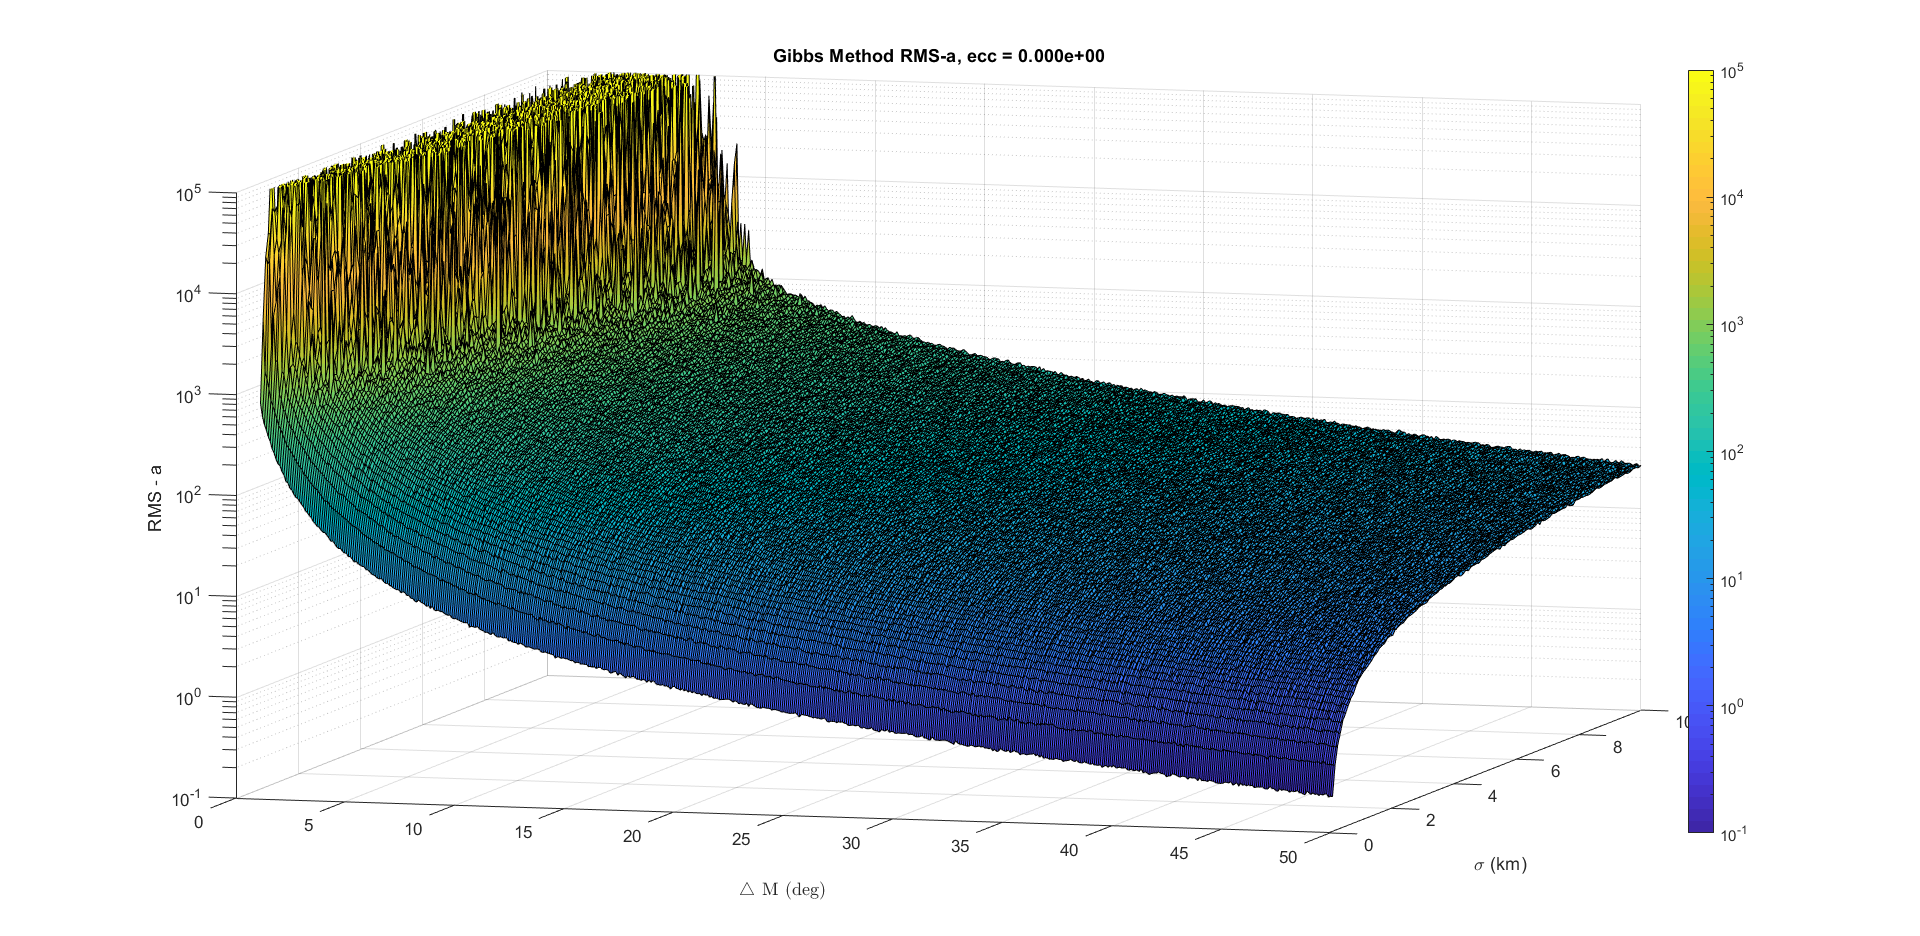
\includegraphics[width=0.7\linewidth]{circularGibbs}
		\caption{RMS error for the semi major axis via Gibbs method for an eccentricity of zero.}
		\label{fig:circulargibbs}
	\end{figure}

	\begin{figure}
		\centering
		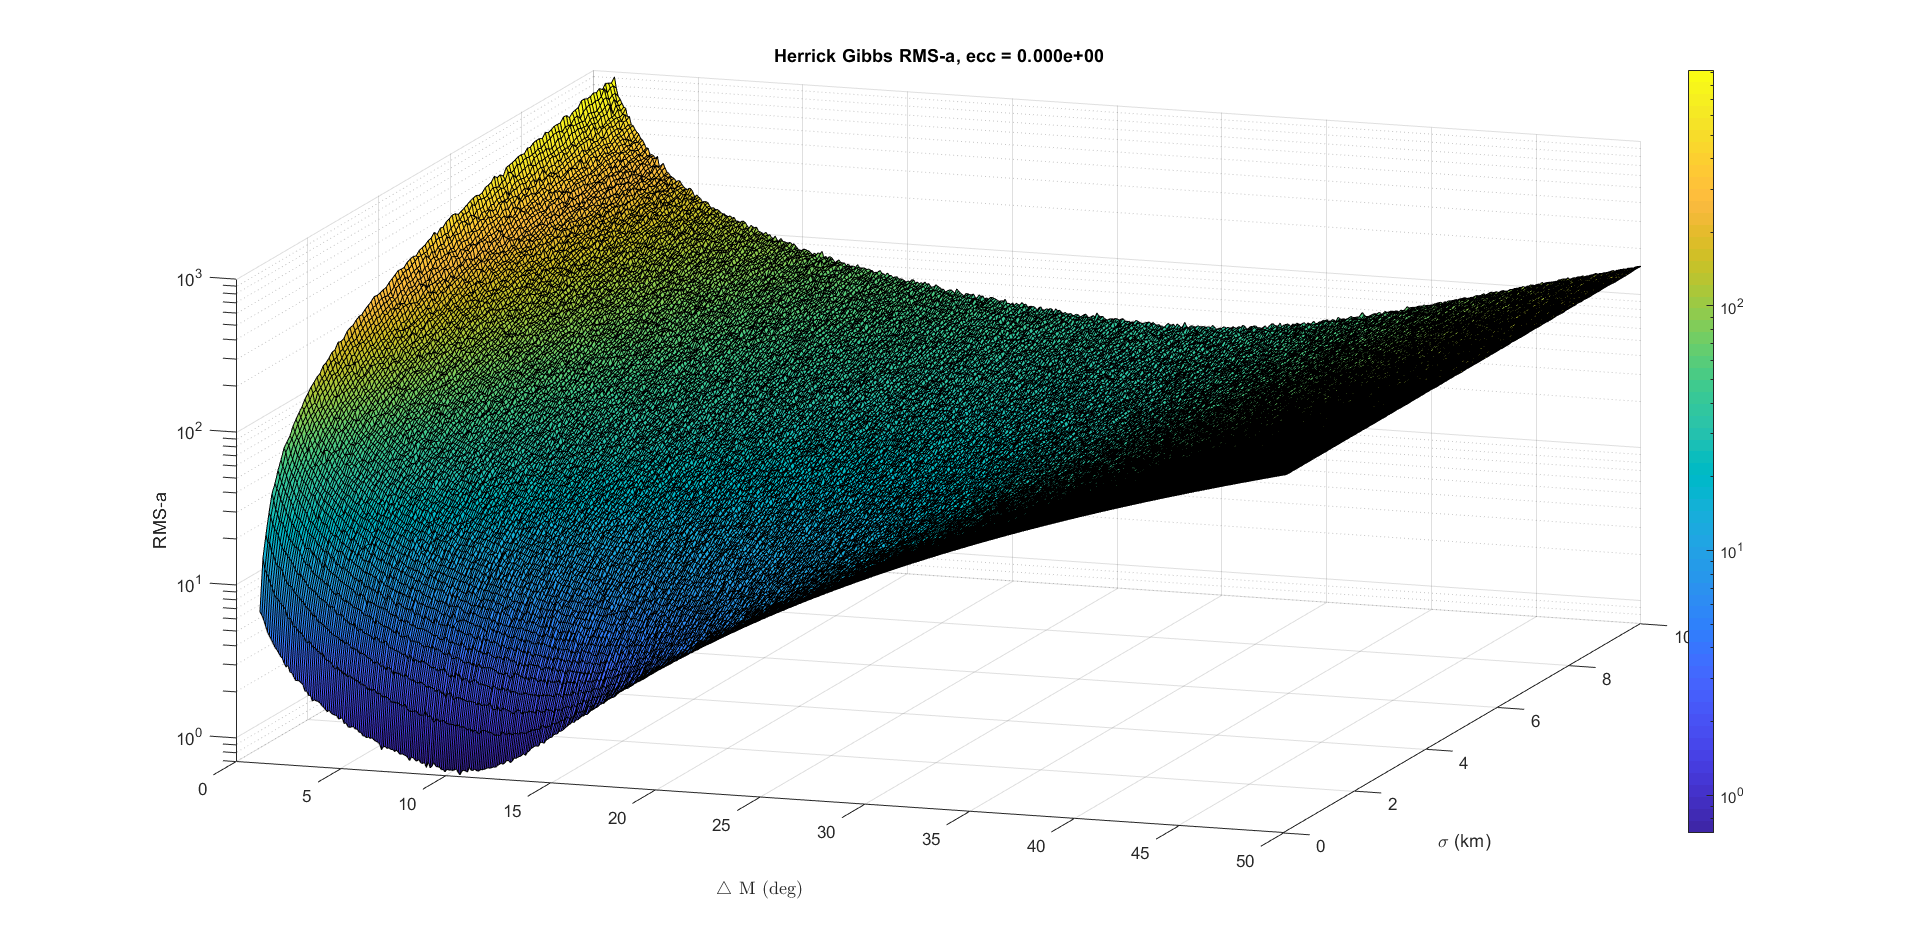
\includegraphics[width=0.7\linewidth]{circularHerrickGibbs}
		\caption{RMS error for the semi major axis via Herrick-Gibbs method for an eccentricity of zero.}
		\label{fig:circularherrickgibbs}
	\end{figure}
\begin{figure}
	\centering
	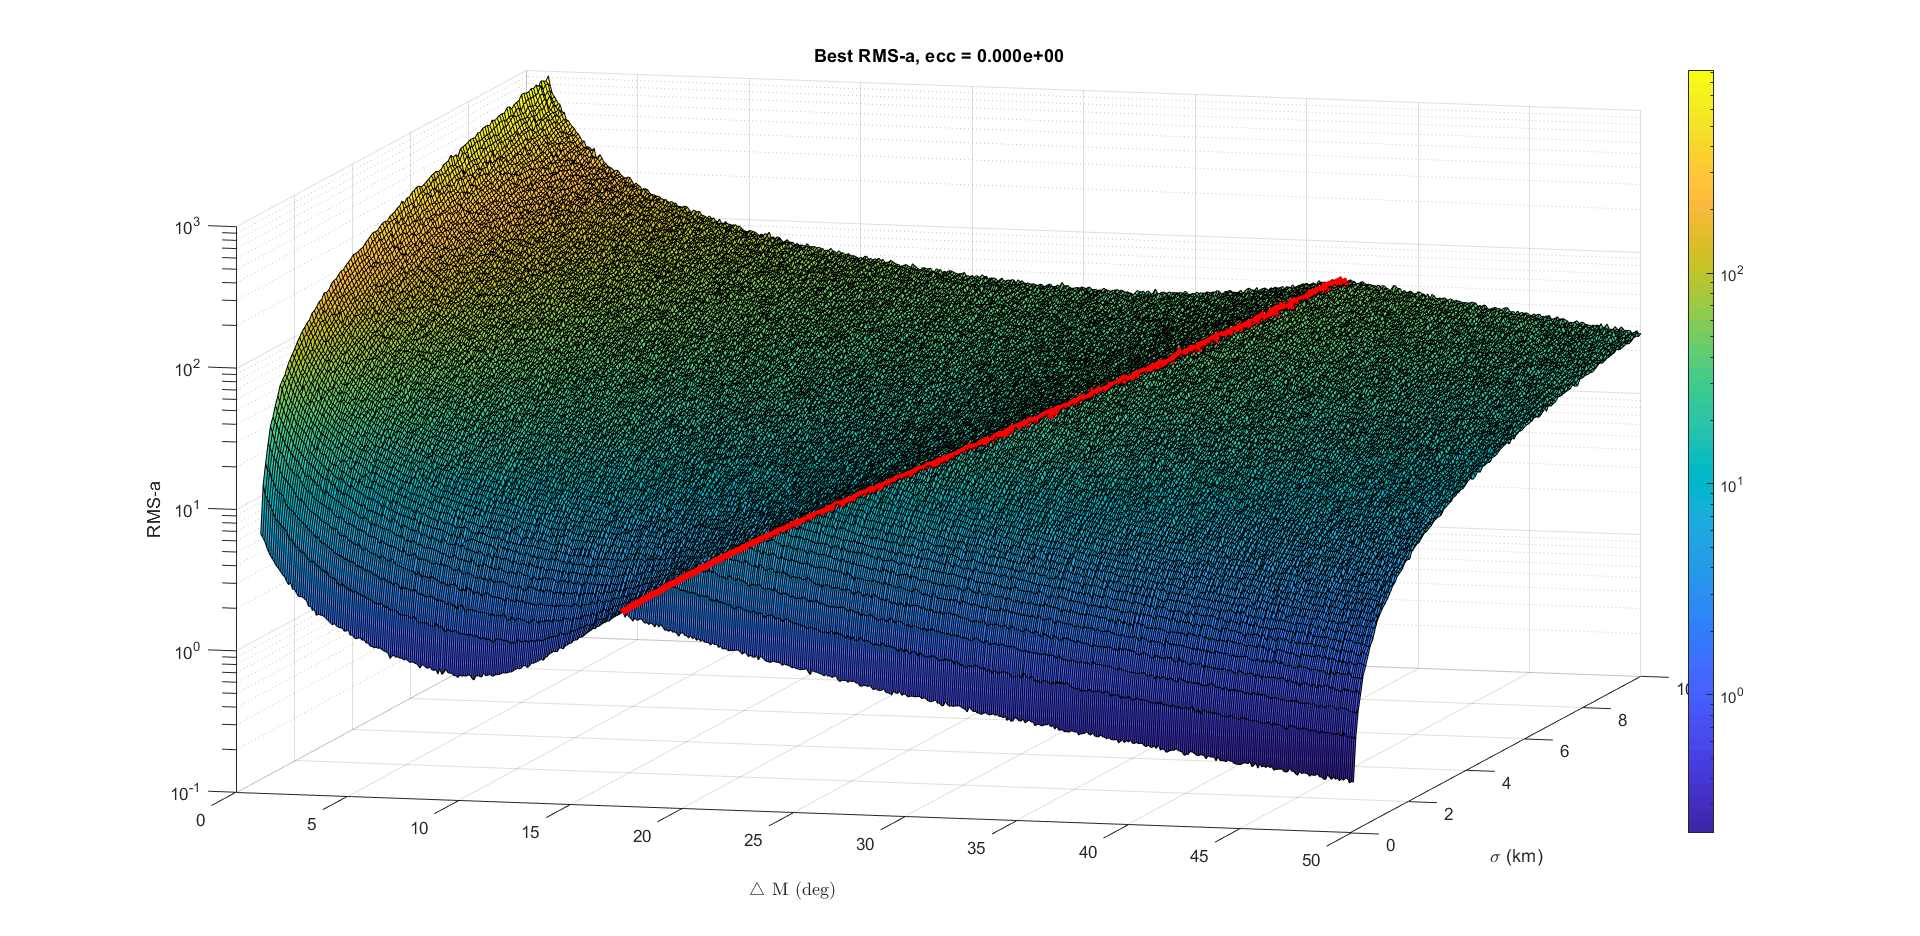
\includegraphics[width=0.7\linewidth]{bestMethodsCirc}
	\caption{The best possible RMS error for the semi major axis. The red line indicates where Gibbs method becomes better than the Herrick Gibbs Method}
	\label{fig:bestmethodscirc}
\end{figure}

	From figure \ref{fig:circulargibbs}, it can be seen that Gibbs method is incredibly inaccurate for position vectors taken within 10 degrees of each other. Herrick-Gibbs however excels in that range. At a low noise level, Gibbs method begins to overtake Herrick Gibbs at a separation of 15 degrees, at a high noise level it takes until 35 degrees of separation for Herrick-Gibbs to be overt taken.
	
	\iffalse
	
	
	For this orbit both methods were run given a range of measurement separation and noise.  over a range of degrees . They were subject to noise
	
	The purpose of this report is to perform an analysis of the Gibbs and Herrick-Gibbs methods of orbital determination when subject to noise. The methods are explained and their derivations given. They are then computed for a sample orbit at various eccentricities. The Root Mean Square Error of both methods is obtained and the accuracy of the methods compared.   and sample sizes. 
	
	
	Going to do a statistical analysis with various eccentricities
	This should be before gibbs
	Then Compare Herrick-Gibbs
	The semi Major will be used
	Or I could use the v2
	I think I should just cut down the size untill I don't have to deal with the asymtote anymore
	Look at what the fund book says for when they are good or no
	
	\section{Results}
	Explain I have a staring orbit
	I go through it for diffrent mean anamolys
	With a a noise
	Then do this for diffrent eccentricities
	Plotting the best of both
	Use the v2 norm, or the a norm?
	Then Look at the change in which method is the most accurate
	
	Purpose of this si not so much the mean anamoly change, but the amount of noise and samples?
	\fi
	These results will be used as a baseline
	
	\subsection{Analysis of Gibbs Method at various eccentricities}
	The following plots come from Gibb's method at an eccentricity of $e=0.05,0.1,0.15$
	\begin{figure}
		\centering
		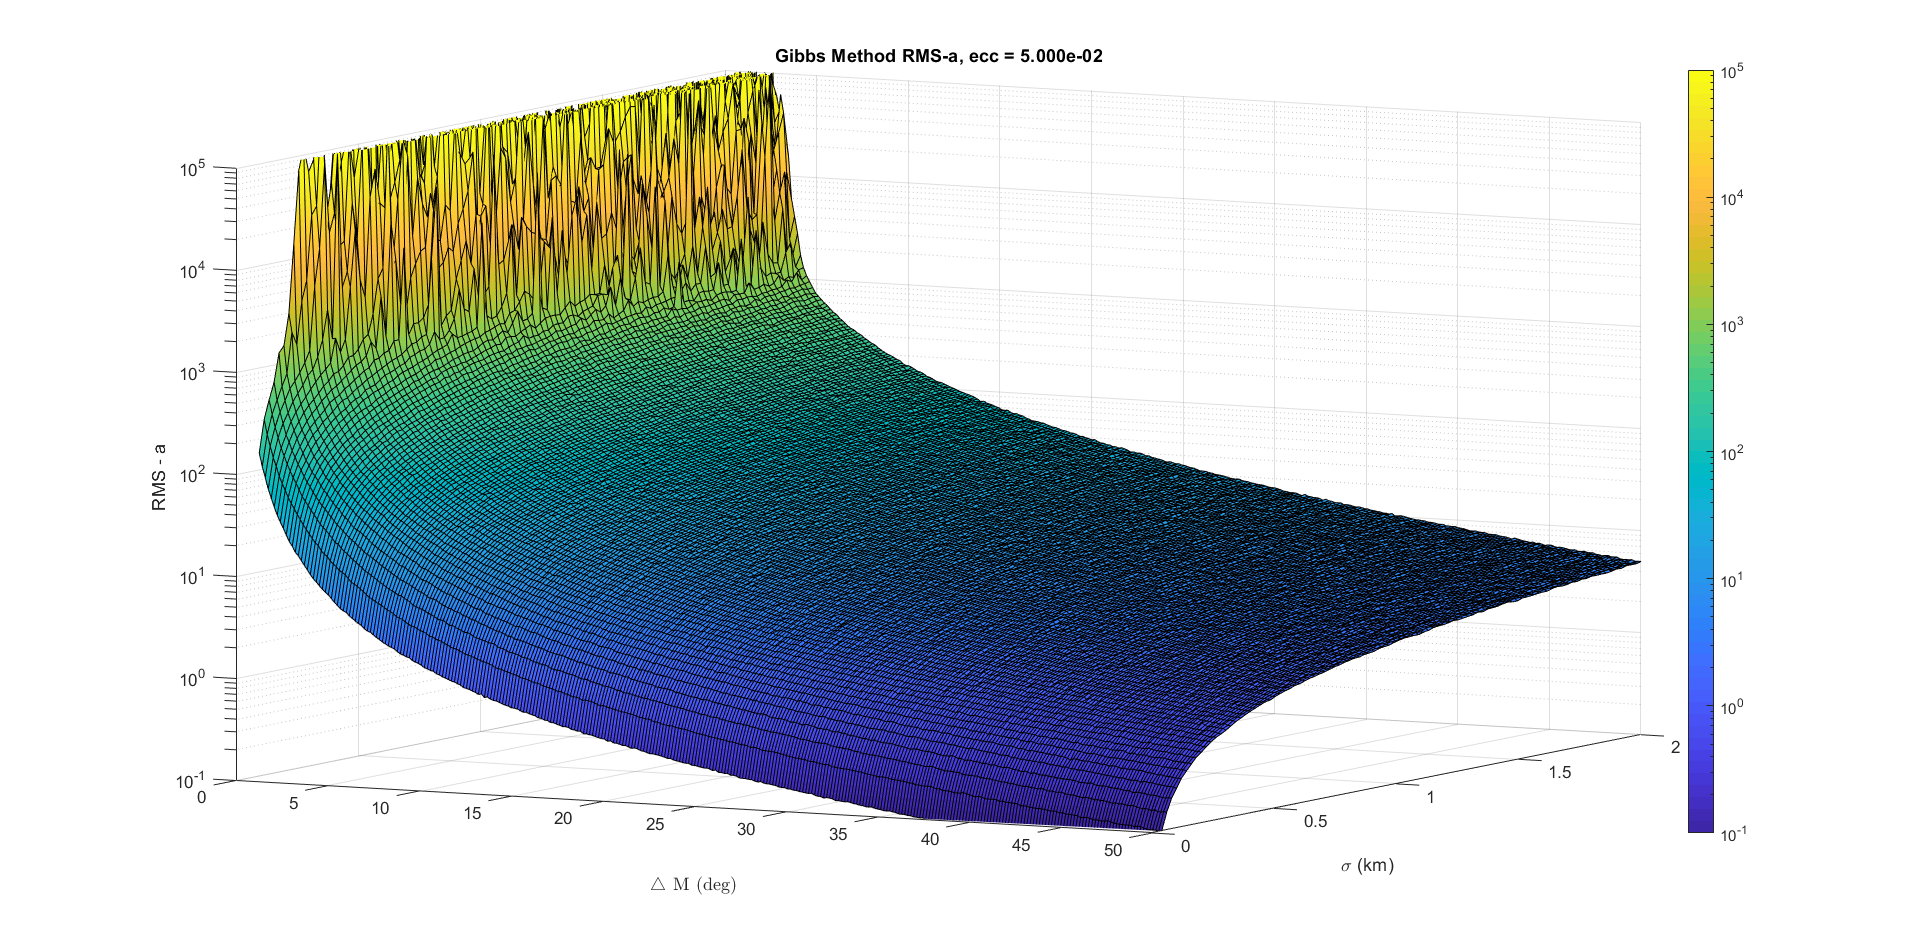
\includegraphics[width=0.7\linewidth]{gibbs_e_05}
		\caption{Gibbs method for an eccentricity of 0.05 vs noise and distance between measurements.}
		\label{fig:gibbse05}
	\end{figure}

	\begin{figure}
	\centering
	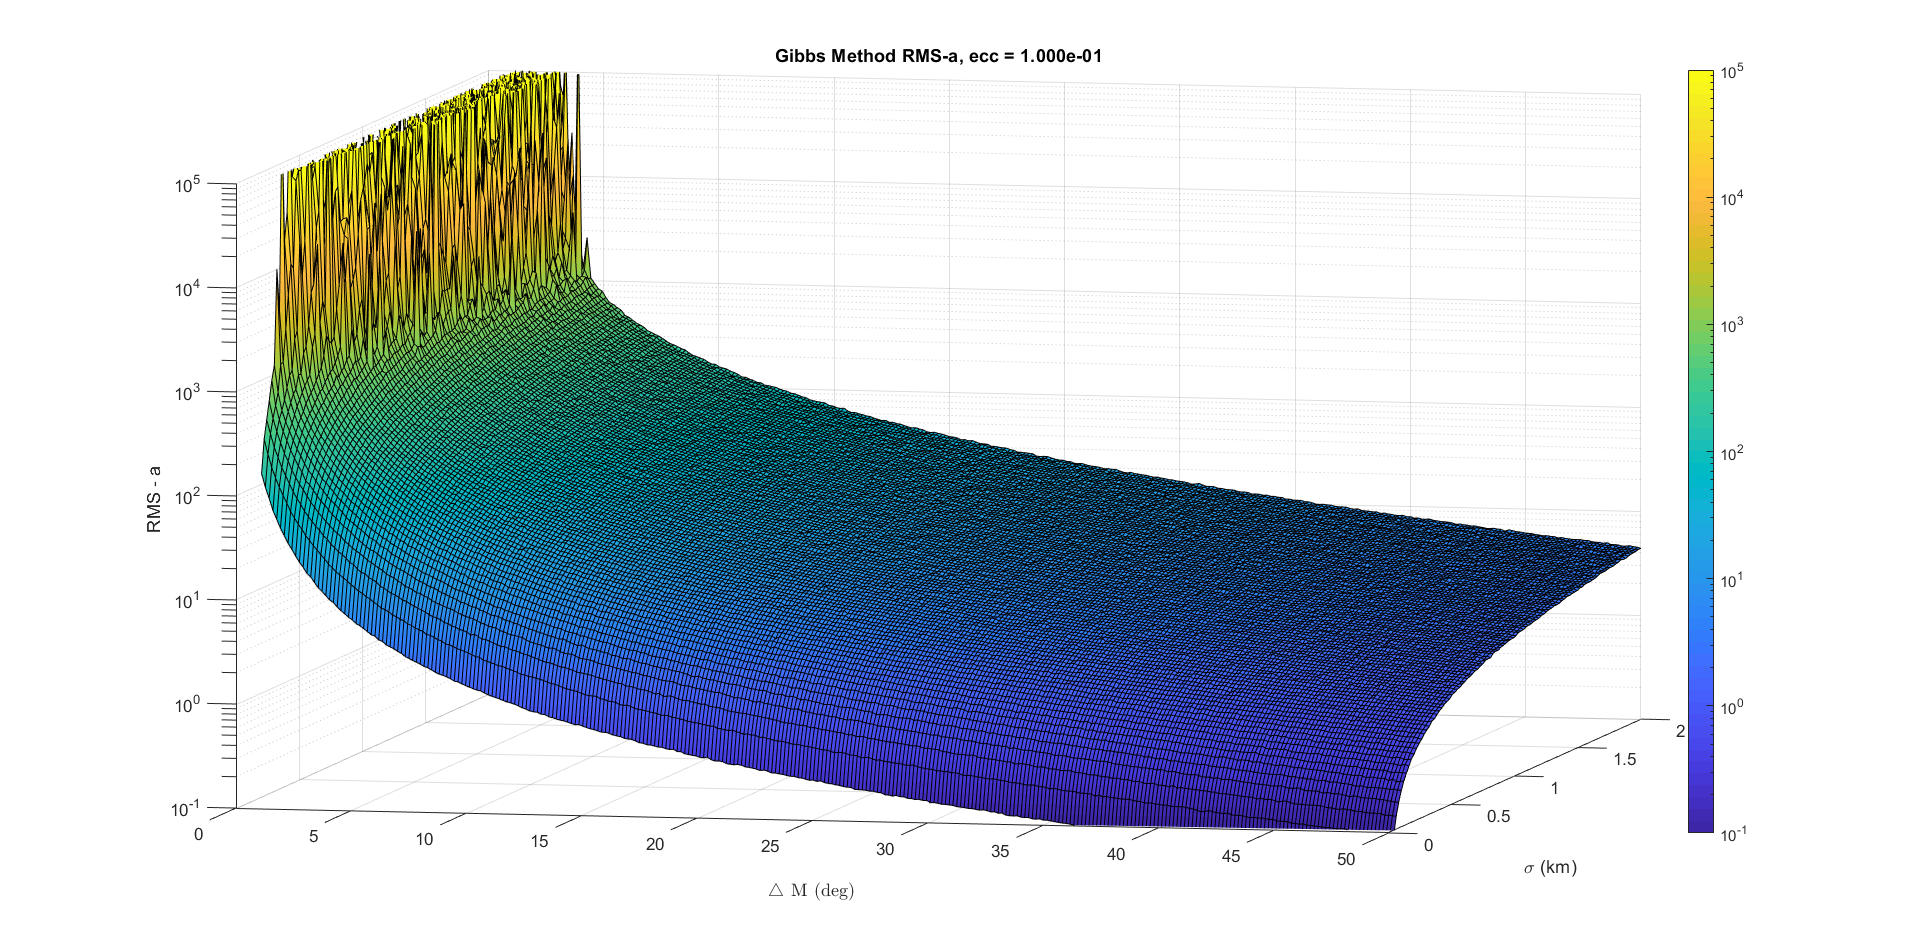
\includegraphics[width=0.7\linewidth]{gibbs_e_1}
	\caption{Gibbs method for an eccentricity of 0.1 vs noise and distance between measurements.}
	\label{fig:gibbse1}
\end{figure}

	\begin{figure}
	\centering
	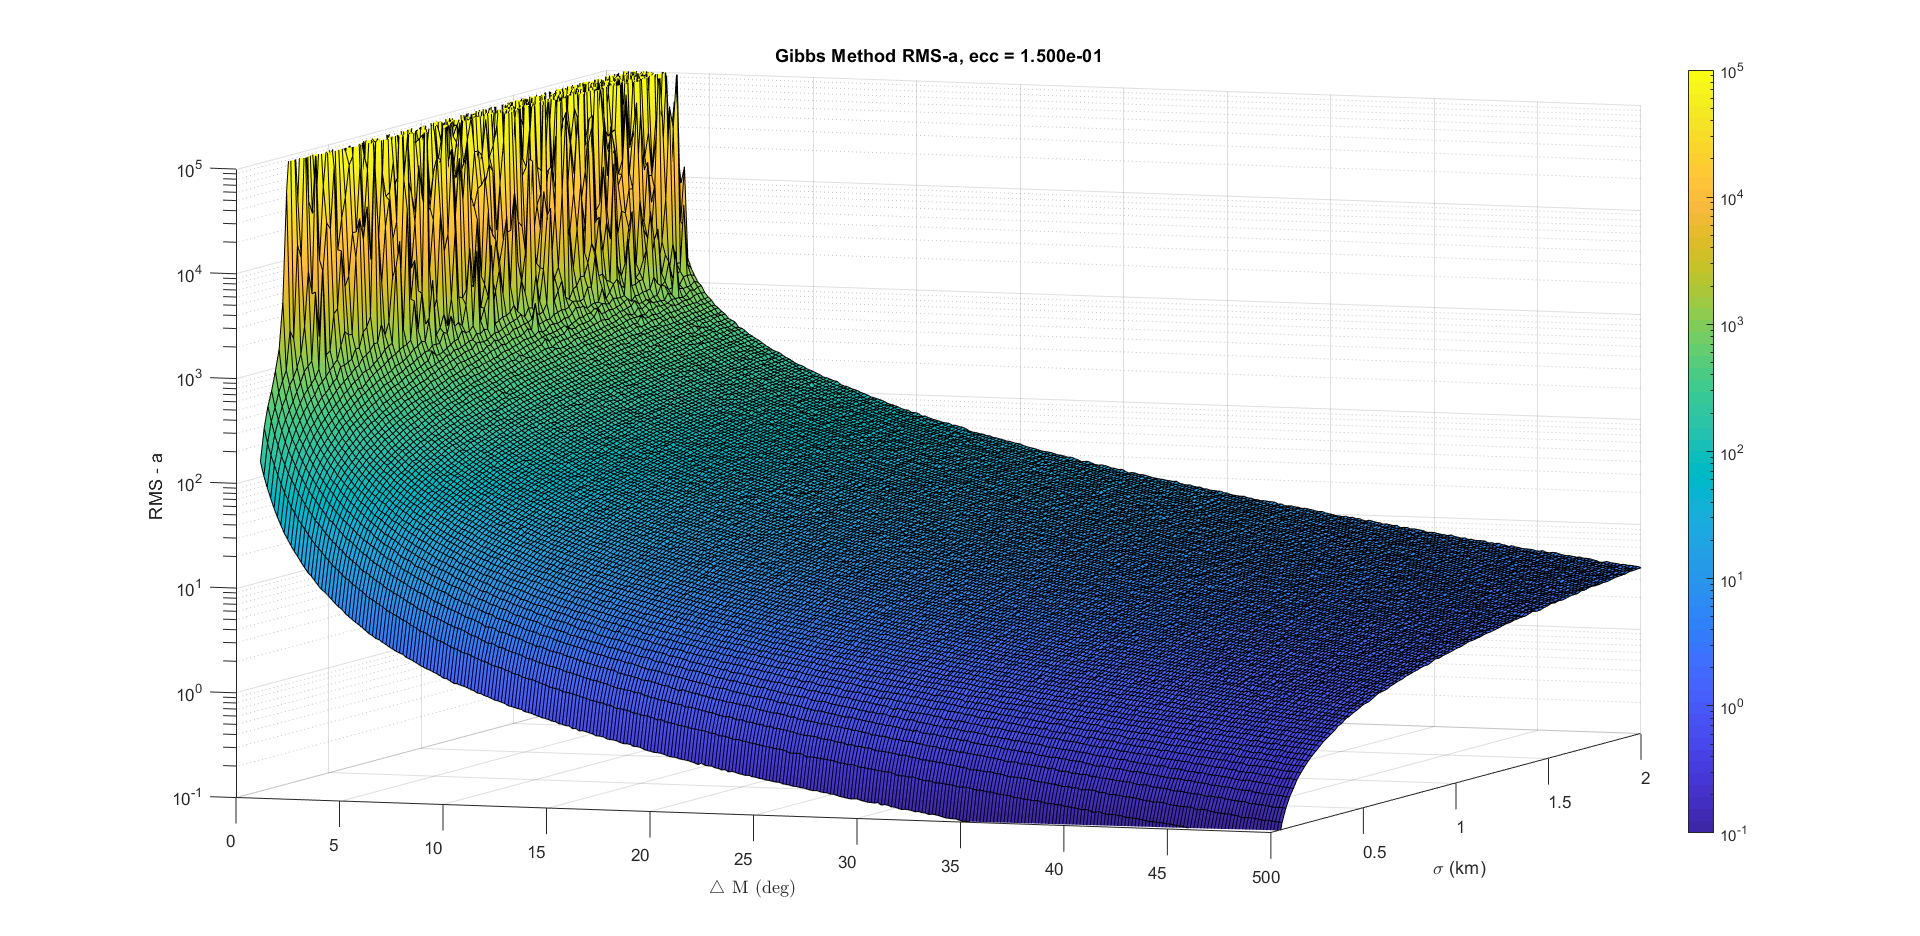
\includegraphics[width=0.7\linewidth]{gibbs_e_15}
	\caption{Gibbs method for an eccentricity of 0.15 vs noise and distance between measurements.}
	\label{fig:gibbse15}
\end{figure}
	
	\newpage
	\subsection{Analysis of Herrick-Gibbs Method at various eccentricities}
		The following plots come from Herrick-Gibb's method at an eccentricity of $e=0.05,0.1,0.15$
		\begin{figure}
		\centering
		\includegraphics[width=0.7\linewidth]{herrickgibbs_e_05}
		\caption{Herrick-Gibbs method for an eccentricity of 0.05 vs noise and distance between measurements.}
		\label{fig:herrickgibbse05}
	\end{figure}
	
	\begin{figure}
		\centering
		\includegraphics[width=0.7\linewidth]{herrickgibbs_e_1}
		\caption{Herrick-Gibbs method for an eccentricity of 0.1 vs noise and distance between measurements.}
		\label{fig:herrickgibbse1}
	\end{figure}
	
	\begin{figure}
		\centering
		\includegraphics[width=0.7\linewidth]{herrickgibbs_e_15}
		\caption{Herrick-Gibbs method for an eccentricity of 0.15 vs noise and distance between measurements.}
		\label{fig:herrickgibbse15}
	\end{figure}
	\subsection{Comparison of methods}
	
	From the previous sections it can be seen  that Gibbs method improves as the distance between observations increases and Herrick-Gibbs method improves up to a point, then decreases in accuracy. We now compare the methods against each other in the following figures 
	\begin{figure}
		\centering
		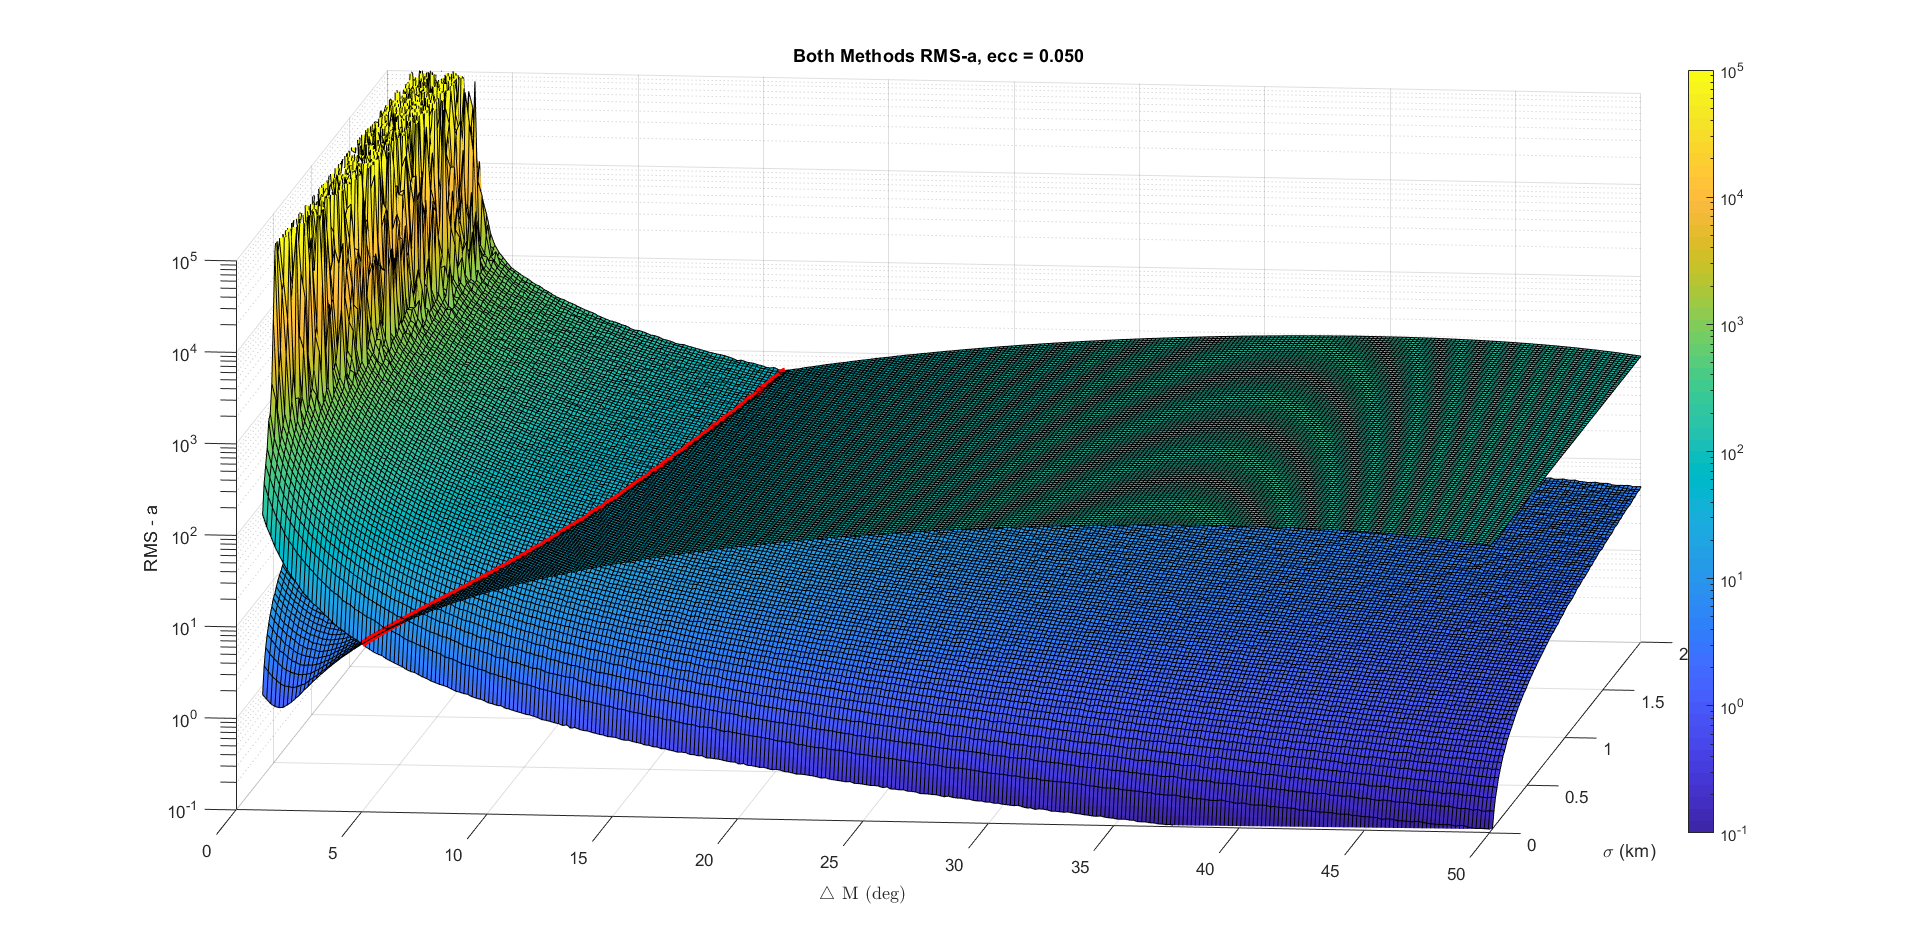
\includegraphics[width=0.7\linewidth]{bothMethods_e_05}
		\caption{Both Gibbs and Herrick-Gibbs at an eccentricity of 0.05}
		\label{fig:bothmethodse05}
	\end{figure}
	\begin{figure}
		\centering
		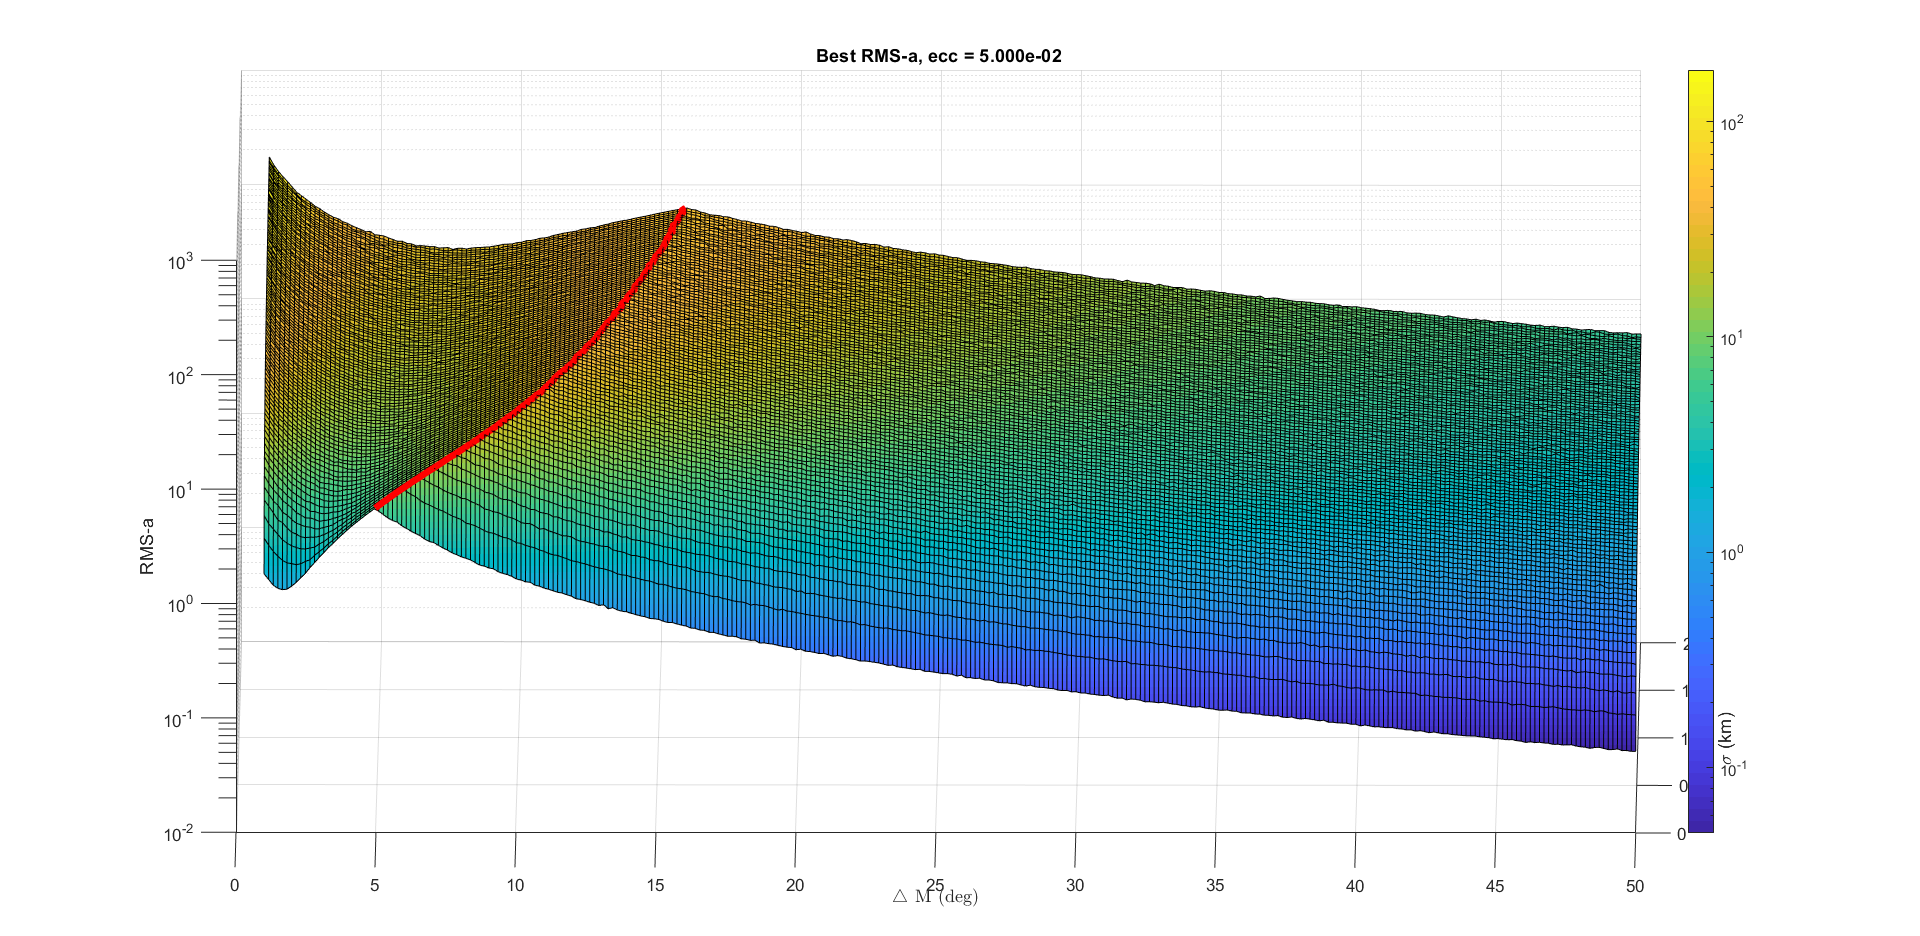
\includegraphics[width=0.7\linewidth]{bestMethods_e_05}
		\caption{The best possible measurement from either method at an eccentricity of 0.05}
		\label{fig:bestmethodse05}
	\end{figure}

	\begin{figure}
	\centering
	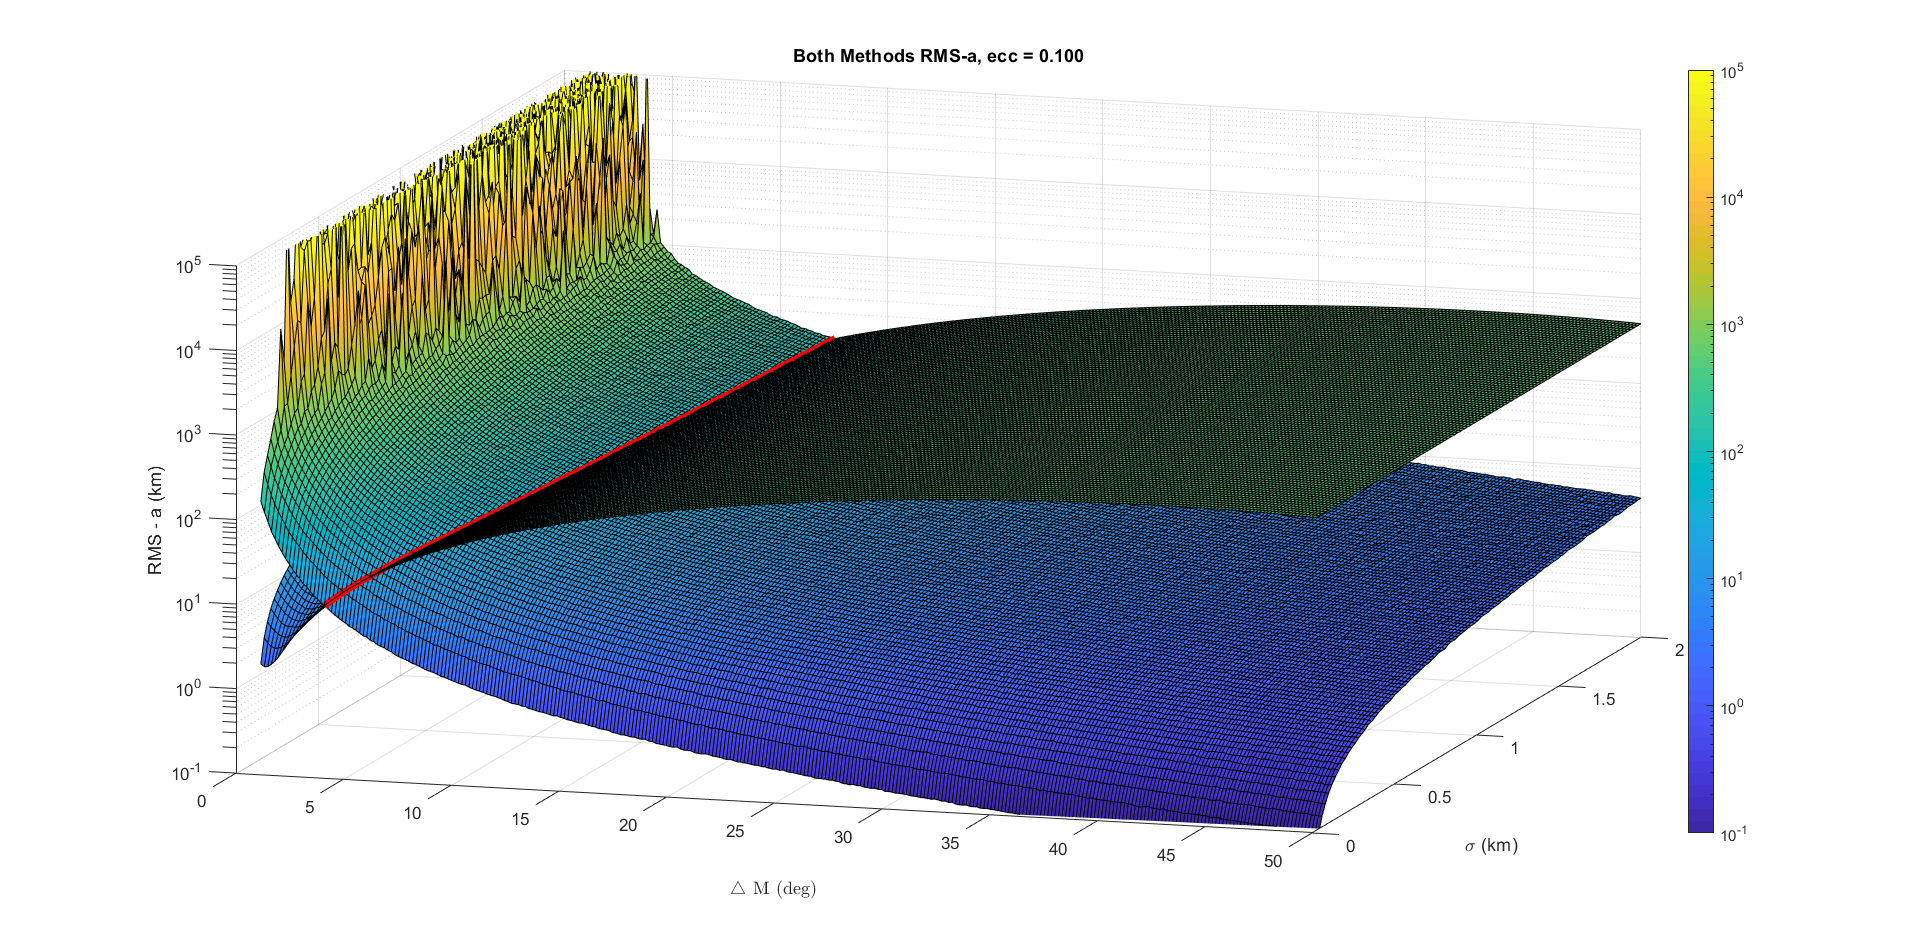
\includegraphics[width=0.7\linewidth]{bothMethods_e_1}
	\caption{Both Gibbs and Herrick-Gibbs at an eccentricity of 0.1}
	\label{fig:bothmethodse1}
\end{figure}
\begin{figure}
	\centering
	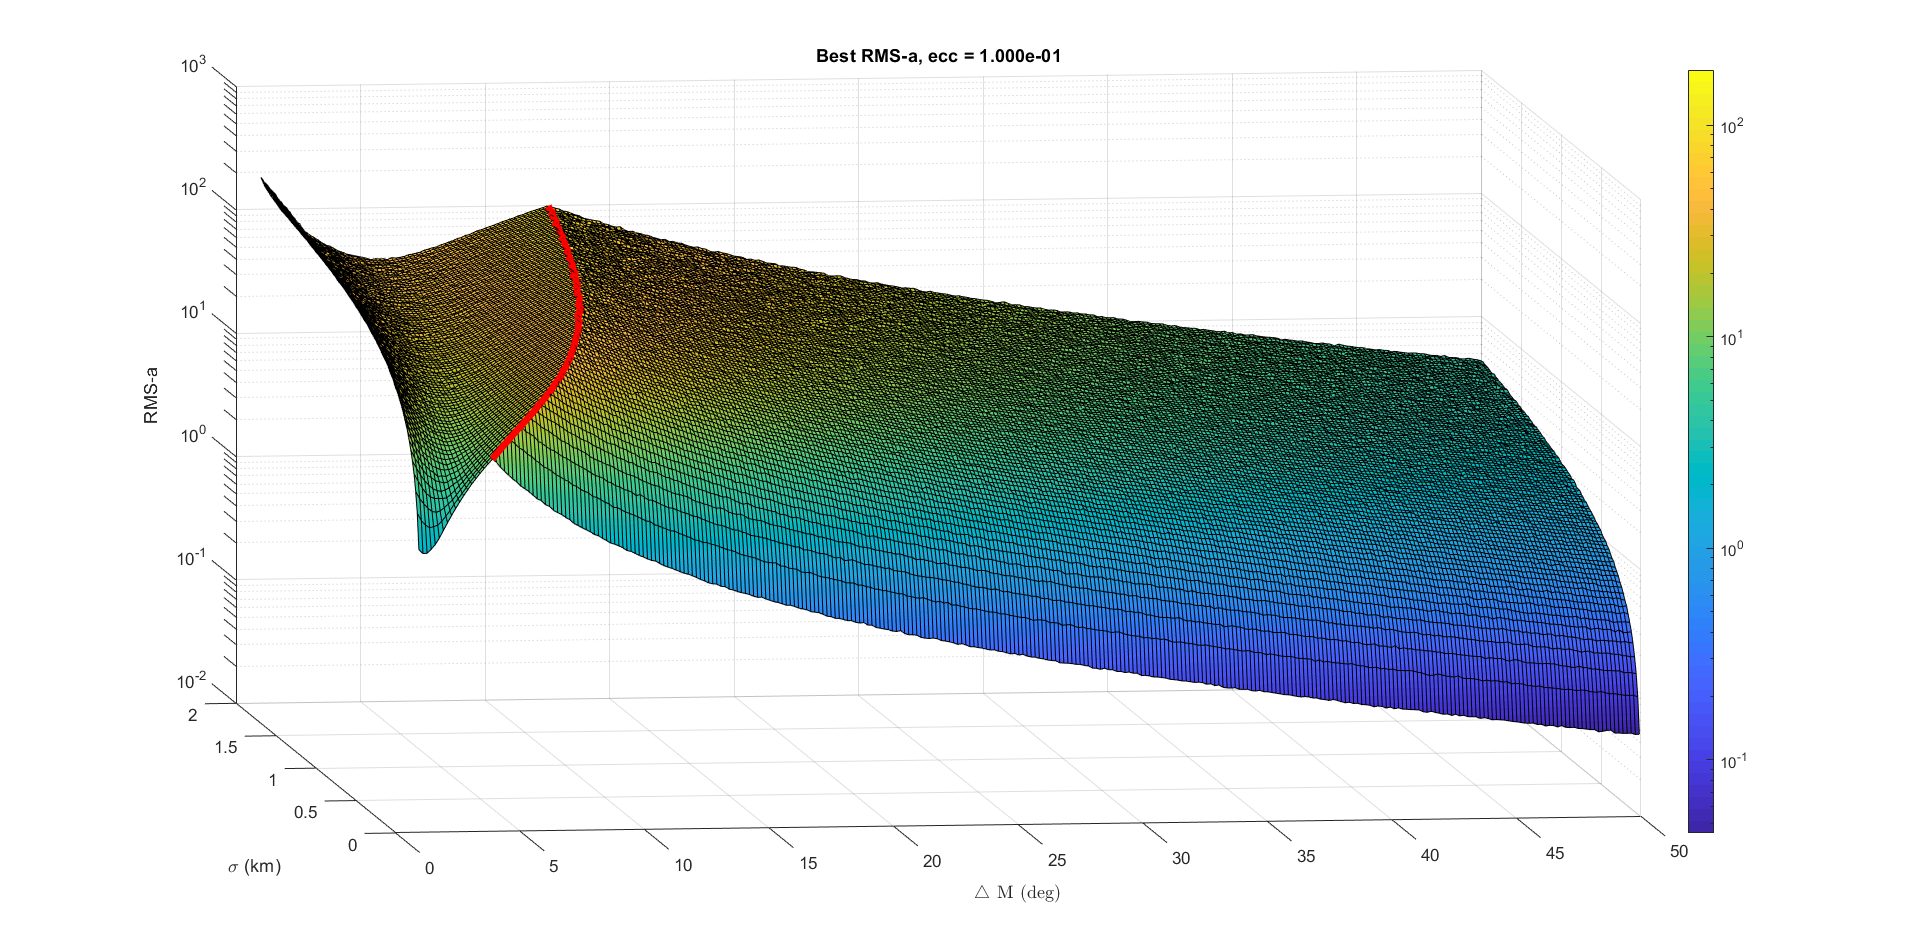
\includegraphics[width=0.7\linewidth]{bestMethods_e_1}
	\caption{The best possible measurement from either method at an eccentricity of 0.1}
	\label{fig:bestmethodse1}
\end{figure}
	\begin{figure}
	\centering
	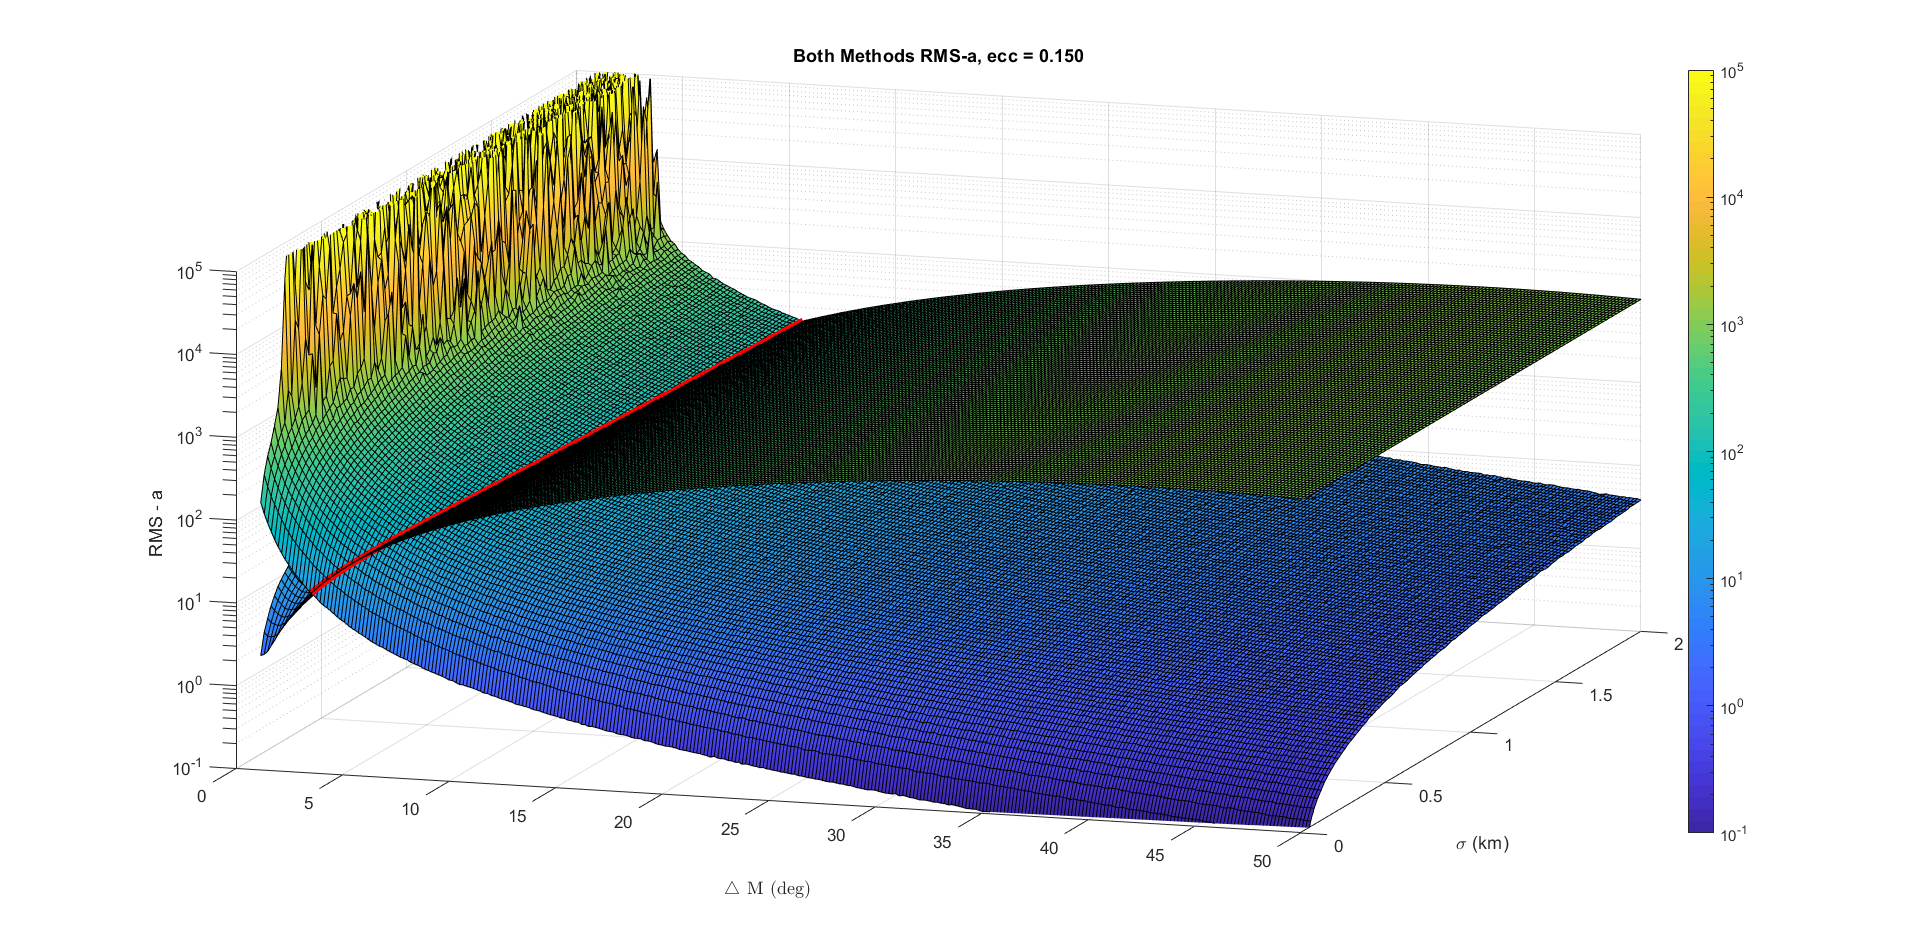
\includegraphics[width=0.7\linewidth]{bothMethods_e_15}
	\caption{Both Gibbs and Herrick-Gibbs at an eccentricity of 0.15}
	\label{fig:bothmethodse15}
\end{figure}
\begin{figure}
	\centering
	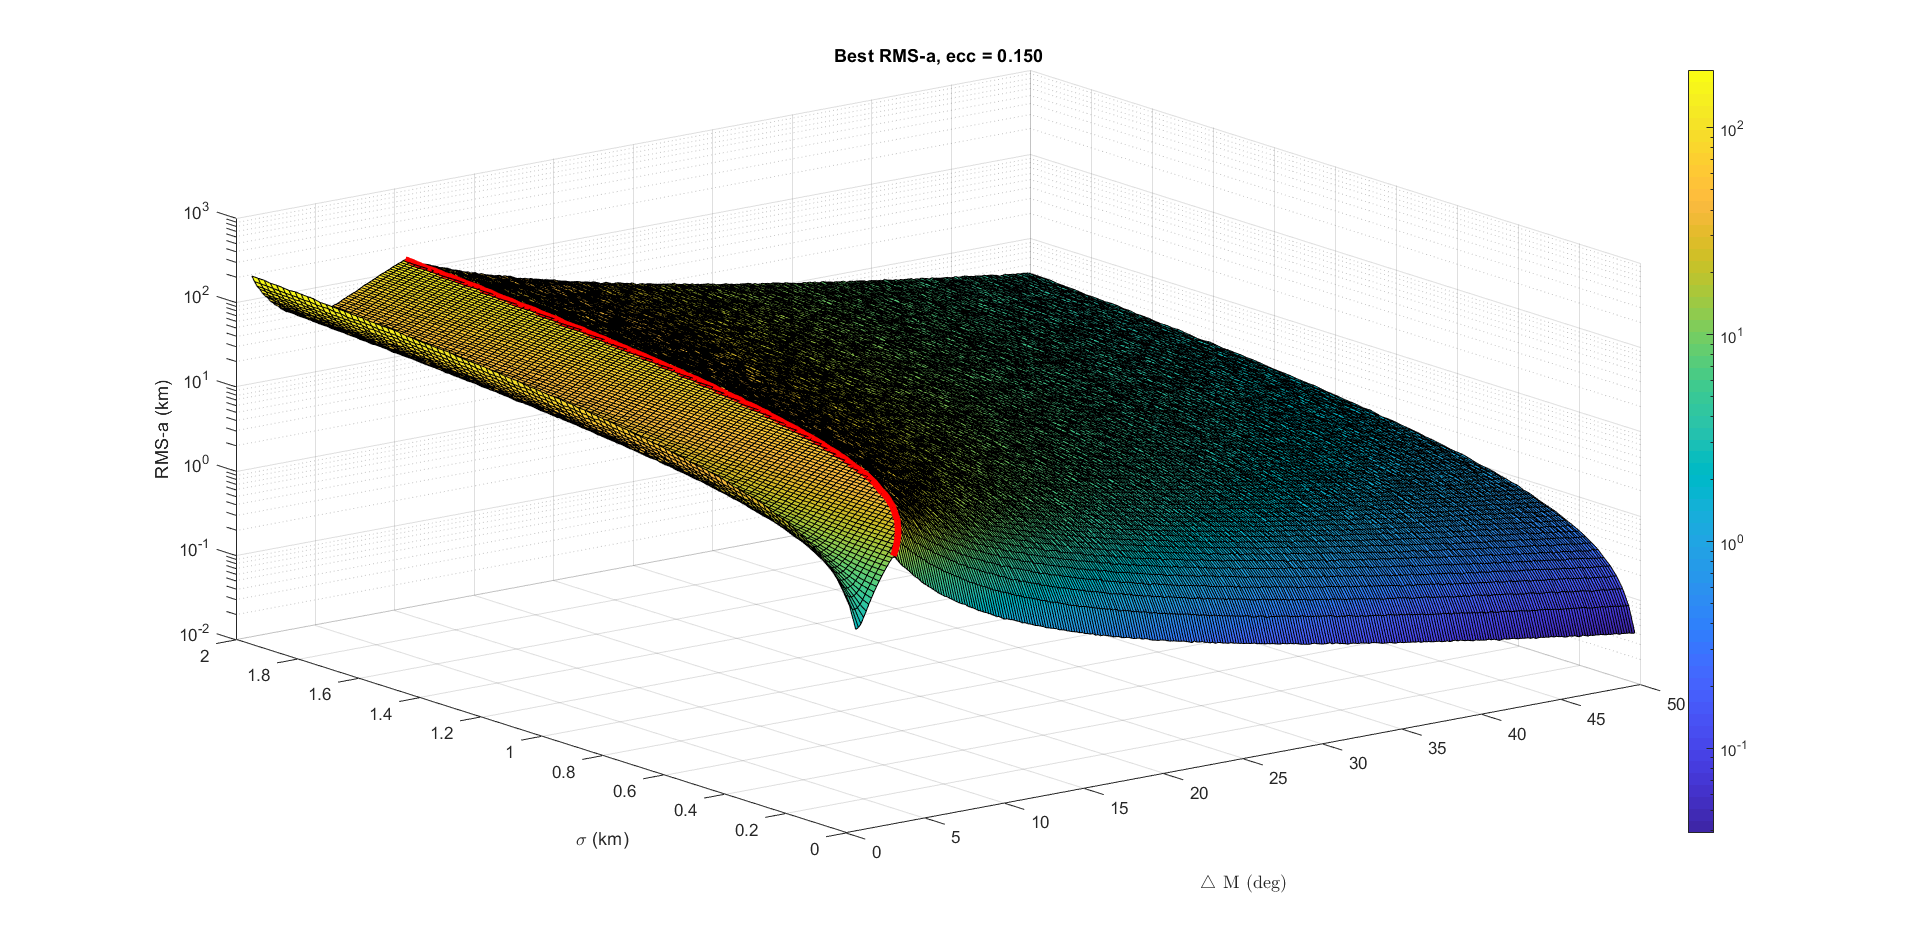
\includegraphics[width=0.7\linewidth]{bestMethods_e_15}
	\caption{The best possible measurement from either method at an eccentricity of 0.15}
	\label{fig:bestmethodse15}
\end{figure}

It becomes clear that Gibbs method remains robust as eccentricity increases, while Herrick-Gibbs does not handle the changes in eccentricity as well. While a circular orbit had Herrick-Gibbs beat Gibbs method for up to 35 degrees between measurements, now Vallado's measurement of 5 degrees seperation has proven accurate for an orbit with an eccentricity of 0.15.\par 


Figure \ref{fig:eccecomp} plots the line where Gibbs method becomes better than Herrick-Gibbs. This provides a more clear demonstration of how as the eccentricity increases, the area  where Herrick-Gibbs is the best method decreases. 
\begin{figure}[H]
	\centering
	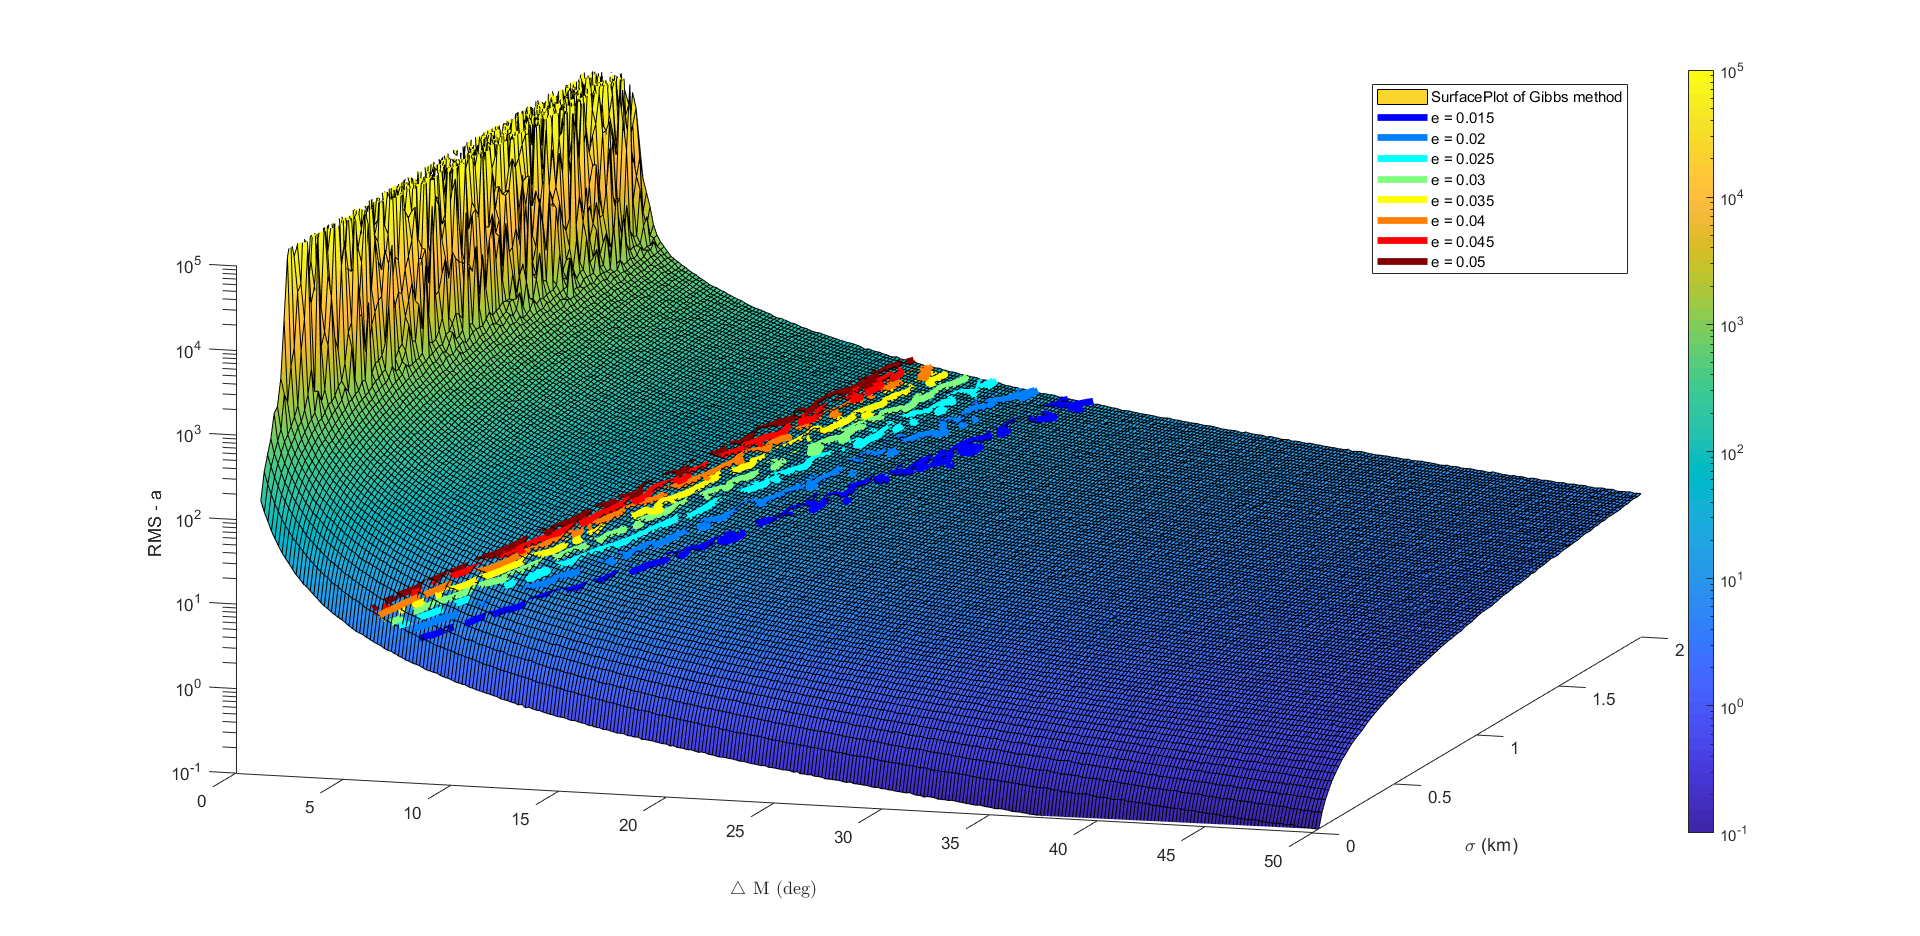
\includegraphics[width=0.7\linewidth]{ecceComp}
	\caption{}
	\label{fig:eccecomp}
\end{figure}




	
	\section{Conclusion}
	\textcolor{red}{ToDo: Finish Conclusions, Upload plots when computer is finished running ,finsh derivation HeckGibb}
		
		%--------------------------------------
		% References
		% -------------------------------------
		
		\bibliographystyle{unsrt}
		\bibliography{ref}

		
		%-----------------------------------------------------------
		% Appendix
		%-----------------------------------------------------------
		\newpage
		\singlespacing
%		\section*{Appendix 1 -derivation of gibbs}
		\section*{Appendix 1 - MATLAB code}
		\addcontentsline{toc}{section}{Appendix}
		
		\lstset{language=Matlab,%
			%basicstyle=\color{red},
			breaklines=true,%
			morekeywords={matlab2tikz},
			keywordstyle=\color{blue},%
			morekeywords=[2]{1}, keywordstyle=[2]{\color{black}},
			identifierstyle=\color{black},%
			stringstyle=\color{mylilas},
			commentstyle=\color{mygreen},%
			showstringspaces=false,%without this there will be a symbol in the places where there is a space
			numbers=left,%
			numberstyle={\tiny \color{black}},% size of the numbers
			numbersep=9pt, % this defines how far the numbers are from the text
			emph=[1]{for,end,break},emphstyle=[1]\color{red}, %some words to emphasise
			%emph=[2]{word1,word2}, emphstyle=[2]{style},    
		}
		
	%\subsection{Master\_TLE.m}
	%\lstinputlisting{C:/Users/Philip/Documents/GitHub/Thesis/Master_TLE.m}
	%\subsection{get\_SATCAT.m}
	%	\lstinputlisting{C:/Users/Philip/Documents/GitHub/Thesis/get_SATCAT.m}
	%	\subsection{get\_TLE\_from\_ID\_Manager.m}
	%\lstinputlisting{C:/Users/Philip/Documents/GitHub/Thesis/get_TLE_from_ID_Manager.m}
	
	%\subsection{get\_TLE\_from\_NorID.m}
	%\lstinputlisting{C:/Users/Philip/Documents/GitHub/Thesis/get_TLE_from_NorID.m}
	%\lstinputlisting{get_SATCAT.m}
	
	%Thanks for Paul McKee who started this template. It seems to have good matlab code viwing
		
	\end{document}
	
